\documentclass[journal, onecolumn, 12pt, draftclsnofoot]{IEEEtran}
\usepackage{breakcites}
\usepackage{graphicx}
\usepackage{amsmath, amsfonts, amssymb}
\usepackage[toc,page]{appendix}

\usepackage{algorithmicx}
\usepackage{algorithm}
\usepackage[noend]{algpseudocode}
\usepackage{bbm}

\usepackage{setspace}
\doublespacing

\usepackage[a4paper, bindingoffset=0.5in,left=1in,right=1in,top=1in,bottom=1in]{geometry}

\newcommand{\kword}[1]{\textbf{#1}}
\newcommand{\mc}[1]{\mathcal{#1}}
\newcommand{\mbf}[1]{\mathbf{#1}}
\newcommand{\E}[2]{\mathbb{E}_{#1} \left[ #2 \right]}

\begin{document}
	\title{Sparse Distributed Memory for Sparse Rewards \\ May 10, 2019}

	%author information
	\author{\IEEEauthorblockN{Alex Van de Kleut} \\
		\IEEEauthorblockA{Department of Neuroscience\\
			Brock University\\
			St. Catharines, Canada\\
			Email: av15fj@brocku.ca} \\ \bigskip
		\IEEEauthorblockN{Sheridan Houghten (Supervisor)} \\
			\IEEEauthorblockA{Department of Computer Science\\
				Brock University\\
				St. Catharines, Canada} \\ \bigskip
		\IEEEauthorblockN{Brian Ross (Co-supervisor)} \\
			\IEEEauthorblockA{Department of Computer Science\\
				Brock University\\
				St. Catharines, Canada} \\
			}

	\maketitle

	\newpage

	\begin{abstract}
		Reinforcement learning is a field of machine learning that involves teaching an agent to maximize rewards from the environment by choosing the best actions. While modern reinforcement learning methods perform very well in environments with dense rewards, they tend to struggle in environments with sparse rewards. This thesis uses Montezuma's Revenge, a 2D puzzle game for the Atari 2600, as a testbed for reinforcement learning in a sparse reward setting. We compare the technique of Random Network Distillation, a method for generating intrinsic reward based on prediction error that achieves state-of-the-art performance in Montezuma's Revenge, to Sparse Distributed Memory, a novel technique that uses recall fidelity as a method for detecting novelty. We find that using Sparse Distributed Memory improves performance over a baseline reinforcement learning agent, but does not achieve state-of-the-art performance.
	\end{abstract}

	\newpage

	\section*{Acknowledgements}
	\par This thesis was completed with the assistance of many researchers and faculty who took the time to assist me with my research. I would like to thank Dr. Sheridan Houghten and Dr. Brian Ross of Brock University's Computer Science department for their continued support with this thesis. I would also like to thank Dr. Pentti Kanerva, who is responsible for the development of Sparse Distributed Memory, for answering questions and providing me with literature material that was not available online. I would like to thank Dr. James Hughes of St. Francis Xavier University who provided an abundance of research ideas and guided me in the research process. Finally, I would like to thank Yuri Burda, the corresponding author for the paper on Random Network Distillation, who clarified for me some implementation details of the paper and allowed me to replicate their results.
	\newpage

	\tableofcontents

	\newpage
	\section{Introduction}
	\label{sec:intro}
	\par This thesis deals with the field of \textbf{reinforcement learning}, a subfield of machine learning and artificial intelligence. In reinforcement learning, there are two main entities: the \textbf{agent} and the \textbf{environment}. The environment is responsible for informing the agent about its current state, and the agent is responsible for responding by choosing an action. In turn, the environment is responsible for changing as a result of that action, and for conferring a reward to the agent corresponding to its choice of action.	We use the notation $s_t$ to refer to the `state' of the environment at some time $t$, the notation $a_t$ to refer to the action taken by the agent at some time $t$, and the notation $r_t$ to refer to the reward given to the agent by the environment for choosing that action in that state. This relationship is visualized in figure \ref{fig:rl}.
	\begin{figure}
		\begin{center}
			\textbf{Reinforcement Learning Loop}
		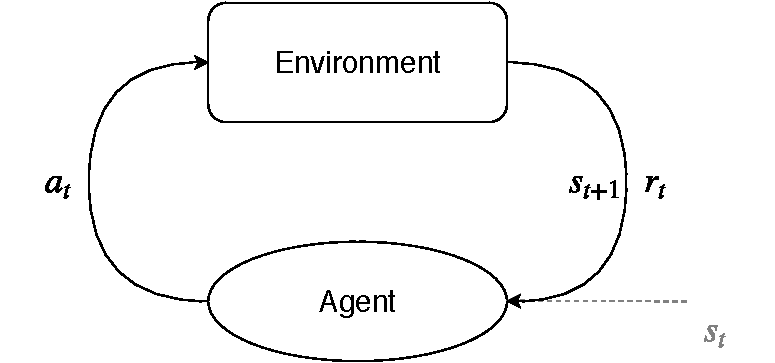
\includegraphics{fig/rl.pdf}
		\end{center}
		\caption{The basic loop of interactions between an agent and its environment in reinforcement learning.}
		\label{fig:rl}
	\end{figure}
	\par Specifically, reinforcement learning is interested in learning \textbf{policies} for the agent (which can be thought of as a set of rules for choosing actions given the current state) that maximize the overall reward.
	\par The focus of this thesis is on methods for learning policies when these rewards are \textbf{sparse}, meaning that they are almost always zero. In a sparse reward setting, the agent does not have a strong learning signal, and so it can be difficult for it to learn a good policy. We discuss the notion of \textbf{intrinsic motivation} and how it can be used to encourage good behaviour environments with sparse rewards.
	\par In section \ref{sec:background}, we build up a rigorous mathematical definition for the relationship between an agent and its environment called a \textbf{Markov Decision Process}. All reinforcement learning makes the basic assumption that an agent is in a Markov decision process. Then, in section \ref{sec:neur}, we compare ideas in neuroscience and psychology to the more formal methods of reinforcement learning, and demonstrate parallels between animal learning and learning policies. In section \ref{sec:q-learning}, we discuss a method for learning a policy called \textbf{$Q$-learning} that learns to choose actions based on a function that predicts how good certain actions in certain states are. In section \ref{sec:policy-gradients}, we discuss a more direct approach to learning a policy by directly modelling the policy as a function that maps states to actions. Specifically, we build up to an understanding of \textbf{Proximal Policy Optimization} and \textbf{Generalized Advantage Estimation} that represent the best-performing general techniques from reinforcement learning available today. In section \ref{sec:intrinsic-motivation}, we discuss the problems with learning in environments with sparse rewards, and describe existing approaches to solving them that have empirically performed well. In section \ref{sec:sdm}, we describe a novel approach to solving intrinsic motivation that involves applying \textbf{Sparse Distributed Memory}; our agent learns to recall which states it has been in in order to encourage exploration. This development is motivated by the fact that current state-of-the-art methods used intrinsic motivation signals that take a significant amount of time to learn (millions ot time steps), whereas sparse distributed memory provides an intelligent intrinsic reward signal essentially instantaneously. In section \ref{sec:methods}, we describe in detail our approach and our implementation of sparse distributed memory and our comparison to current state-of-the-art, using a sparse reward environment called \textbf{Montezuma's Revenge}, a videogame for the Atari 2600 as a testbed. In section \ref{sec:results}, we report our results compared to the state-of-the-art, a baseline that uses no intrinsic motivation, and a random agent. In section \ref{sec:discussion}, we consider the possibilities for why the agent using sparse distributed memory achieves the level of performance that it does, and discuss directions for future work.

	\newpage
	\section{Background}
	\label{sec:background}
	\par The field of reinforcement learning in computer science is historically rooted in the field of operant conditioning from psychology. Operant conditioning is a technique to used modify behaviour through the use of reward and punishment: behaviour should increase in frequency when associated with the addition of a positive stimulus or the removal of a negative stimulus, and should decrease in frequency when associated with the removal of a positive stimulus or the addition of a negative stimulus \cite{operant_conditioning}.
	\par From this, reinforcement learning researchers have gleaned a guiding principle that informs every development in the field: the \kword{reward hypothesis}. The reward hypothesis states that \textit{every action of a rational agent can be thought of as seeking to maximize some cumulative scalar reward signal} \cite{reward_hypothesis}. The reward hypothesis is foundational to reinforcement learning, since it gives us a basic framework for designing agents that behave rationally.
	\par Reinforcement learning relies heavily on its theoretical foundations. Problems in reinforcement learning are framed as \kword{Markov Decision Processes} (MDPs). MDPs are extensions of stochastic models known as \kword{Markov Processes} \cite{rl}.

		\subsection{Markov Processes}
		\par A Markov Process is, formally, a tuple $\langle \mc{S}, \mc{P} \rangle$ where $\mc{S}$ is a set of states and $\mc{P} : \mc{S}^2 \to [0, 1]$ is a function describing the probability of transitioning from state $s$ to state $s'$:
		\begin{equation}
			\label{eqn:state_transition_probability}
			\mc{P}(s,s') = \mathbb{P} \left[s' \big\vert s \right]
		\end{equation}

		 \par Markov processes are used to model stochastic sequences of states $s_1, s_2, \dots, s_T$ satisfying the \kword{Markov Property}:

	\begin{equation}
		\label{eqn:markov_property}
		\mathbb{P}\left[ s_{t+1} \big\vert s_t \right] = \mathbb{P}\left[ {s_{t+1} \big\vert s_1, s_2, \dots, s_t} \right]
	\end{equation}
	that is, the probability of transition from state $s_t$ to state $s_{t+1}$ is independent of previous transitions.
	\subsection{Markov Reward Processes}
	\par A \kword{Markov Reward Process} is an extension of a Markov Process that allows us to associate rewards with states. Formally, it is a tuple $\langle \mc{S}, \mc{P}, \mc{R} \rangle$ that allows us to associate with each state transition $\langle s_t, s_{t+1} \rangle$ some reward
	\begin{equation}
		\label{eqn:reward_process}
		\mc{R}(s_t, s_{t+1}) = \mathbb{E}\left[r_t \big\vert s_t, s_{t+1} \right]
	\end{equation}
	which is often simplified to being $\mc{R}(s_t)$, the reward of being in a particular state $s_t$.
	\par Consider a \kword{trajectory} $\tau$ of transitions
	$$\tau = \langle s_t, s_{t+1}, s_{t+2}, \dots, s_{T} \rangle $$
	visited in a Markov reward process, associated with a sequence of rewards
		$$
		\langle r_t, r_{t+1}, r_{t+2}, \dots, r_{T} \rangle
		$$
	Then according to the reward hypothesis, we should be interested in trajectories that maximize the \kword{return} $R_t$:
	\begin{align}
		\label{eqn:undiscounted_rewards}
		R_t &= r_t + r_{t+1} +  r_{t+2}+  \dots + r_T  \\
		&= \sum_{k=t}^T r_k \nonumber
	\end{align}
	\par When $T$ is finite, we say that the trajectory has a \kword{finite time horizon} and that the environment is \kword{episodic} (happens in `episodes').
	\par For infinite time horizons, we cannot guarantee that $R_t$ converges. As a result, we might consider discounting rewards exponentially over time in order to guarantee convergence. This line of reasoning leads us to the \kword{discounted return} $G_t$:
	\begin{align}
		\label{eqn:G}
		G_t &= r_{t} + \gamma r_{t+1} + \gamma^2 r_{t+2} + \dots \\
		&= \sum_{k=t}^\infty \gamma^{k-t} r_k \nonumber
	\end{align}
	where $\gamma$ is a discount factor between $0$ and $1$ (often close to $1$).
	\par We sometimes refer to both the discounted and undiscounted return as just `return' for brevity, and write $G_t$ where for some episodic environments it may be more appropriate to use $R_t$. In fact, it should not be hard to see that $R_t$ is just $G_t$ with $r_t = 0$ for $t > T$ and $\gamma = 1$.

	\subsection{Value Function}
	\par We can use the expected value of $G_t$ to determine the \kword{value} of being a certain state $s$:
	\begin{equation}
		\label{eqn:value}
		V(s_t) = \mathbb{E}\left[ G_t \big\vert s_t \right]
	\end{equation}

	We can decompose $V(s_t)$ into two parts: the immediate reward $r_t$ and the discounted value of being in the next state $s_{t+1}$:
	\begin{align}
		\label{eqn:bellman}
		\begin{split}
			V(s_t) &= \mathbb{E} \left[ G_t \big\vert s_t \right] \\
					&= \mathbb{E} \left[ r_{t} + \gamma r_{t+1} + \dots + \gamma^2 r_{t+2} \big\vert s_t \right] \\
					&= \mathbb{E}\left[r_{t} + \gamma (r_{t+1} + \gamma r_{t+2} + \dots) \big\vert s_t \right] \\
					&= \mathbb{E}\left[ r_{t} + \gamma G_{t+1} \big\vert s_t \right] \\
					&= \mathbb{E} \left[ r_{t} + \gamma V(s_{t+1}) \big\vert s_t \right] \\
		\end{split}
	\end{align}

	The last form of $V(s_t)$ in (\ref{eqn:bellman}) is known as the \kword{Bellman Equation}.

	\subsection{Markov Decision Processes}
	\par A \kword{Markov Decision Process} (MDP) is an extension of a Markov Reward Process that allows state transitions to be conditional upon some action. Formally, it is a tuple $\langle \mc{S}, \mc{A}, \mc{P}, \mc{R} \rangle$ where $\mc{A}$ is a set of actions available to an agent in a state $s_t$. We reformulate (\ref{eqn:reward_process}) as follows:
		\begin{equation}
			\label{eqn:decision_process}
			\mc{R}(s_t, a_t) = \mathbb{E}\left[r_{t} \big\vert s_t, a_t \right]
		\end{equation}

		\par This is the model we will use to describe problems in reinforcement learning. In this case, state transitions now include the action taken:
		$$\langle s_t, a_t, s_{t+1} \rangle$$
		and that trajectories $\tau$ are now of the form
		$$\langle s_t, a_t, s_{t+1}, a_{t+1}, \dots \rangle$$
		We must also update $\mc{P}$ to be the probability of transitioning to state $s_{t+1}$ given that the current state is $s_t$ and the current action is $a_t$.
		\begin{equation}
			\label{eqn:state_transition_probability_MDP}
			\mc{P}(s_t,a_t,s_{t+1}) = \mathbb{P}\left[s_{t+1} \big\vert s_t, a_t \right]
		\end{equation}
		Whereas in an MRP the probability of generating trajectories is dependant upon only the dynamics of the underlying Markov process, in an MDP trajectories also depend on the actions of an agent. For an example of an MDP, see figure \ref{fig:mdp}.
		\begin{figure}
			\begin{center}
			\textbf{Markov Decision Process} \\
			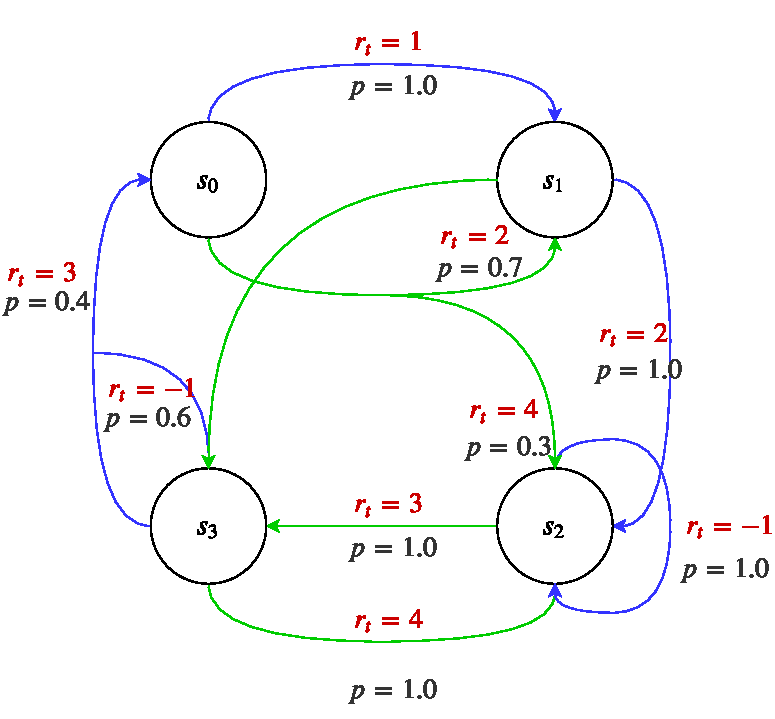
\includegraphics{fig/mdp.pdf}
			\end{center}
			\caption{An example of a Markov Decision Process with four states: $s_0, s_1, s_2, s_3$ and two actions, in green and blue. For each action, we show the probability of transitioning to another state given the current state and the chosen action, as well as the associated reward for that transition. For transitions with probability $0$, we do not write an arrow. For many transitions, the probability of transitioning is $1$, but for some, the next state given the current state and the current action might be probabilistic, such as the transition from $s_0$ taking the green action.}
			\label{fig:mdp}
		\end{figure}

		\subsection{Policies}
		\par Our goal is to design an agent capable of behaving rationally, that is, capable of maximizing the return. In the context of MDPs, this means having a strategy for choosing an action $a_t$ given the state $s_t$. We call this the \kword{policy} of the agent.
		\par There are two kinds of of policies: \kword{deterministic policies} are policies that directly map states to actions, and are usually denoted $\mu$:
		\begin{equation}
			\label{eqn:mu-deterministic-policy}
			\mu: \mc{S} \to \mc{A}
		\end{equation}
		where we have $a_t = \mu(s_t)$.
		\par The second kind of policies are \kword{stochastic policies} that form a probability distribution over possible actions that can be taken, and are usually denoted $\pi$:
		\begin{equation}
			\label{eqn:pi-nondeterministic-policy}
			\pi: \mc{S} \times \mc{A} \to [0,1]
		\end{equation}
		where we have $a_t \sim \pi ( \cdot \big\vert s_t)$.
		\par In general we can refer to a policy as $\pi$ since we can regard $\mu$ is a special case where the probability distribution collapses around a single action.

		Given a policy $\pi$, an agent can now choose actions at each state to shape the sequences of states that it visits. We thus have a new formulation of the value function (\ref{eqn:value-return}):
		\begin{equation}
			\label{eqn:value-return}
			V^\pi(s_t) = \mathbb{E}_\pi \left[ G_t \big\vert s_t \right]
		\end{equation}
		which can be thought of as the expected value of starting in state $s_t$ and choosing actions in subsequent states according to the policy $\pi$.
		\subsection{Action-Value Function}
		\par We can extend our redefined function (\ref{eqn:action-value}) to consider the expected return of taking action $a_t$ in state $s_t$ and from there following the policy $\pi$ at each subsequent state.
		\begin{equation}
			\label{eqn:action-value}
			Q^\pi(s_t,a_t) = \mathbb{E}_\pi \left[ G_t \big\vert s_t, a_t \right]
		\end{equation}
		Whereas $V^\pi(s_t)$ associates a `goodness' with a state $s_t$ according to a policy $\pi$, $Q^\pi(s_t,a_t)$ describes the \kword{quality} of taking an action $a_t$ in a state $s_t$.
		\par Just as in (\ref{eqn:bellman}), we can decompose $Q^\pi(s_t,a_t)$ as follows:
		\begin{equation}
			\label{eqn:q_bellman}
			Q^\pi(s_t,a_t) = \mathbb{E}_\pi \left[ r_t + \gamma Q^\pi(s_{t+1}, a_{t+1}) \big\vert s_t, a_t \right]
		\end{equation}
		Since the value function is the expected reward for choosing an action $a_t$ starting in state $s_t$ according to the policy $\pi$, we can see that
		\begin{equation}
			\label{eqn:value-as-expectation-over-action-value}
			V^\pi(s_t) = \mathbb{E}_{a_t \sim \pi} \left[ Q^\pi(s_t, a_t) \big\vert s_t \right]
		\end{equation}
		\subsection{Optimal Policy}
		\par Under the paradigm of the $Q$ function, what does it mean for an agent to have an \kword{optimal policy}? An optimal policy $\pi^*$ should satisfy the optimal value function:
		\begin{equation}
			\label{eqn:optimal-value-function}
			Q^*(s_t,a_t) = \max_{\pi} \mathbb{E}_\pi \left[ r_t + \gamma Q^*(s_{t+1}, a_{t+1}) \big\vert s_t, a_t \right]
		\end{equation}
		that is, it should choose actions that maximize the expected return over a trajectory. Then from this we can derive a greedy optimal policy:
		\begin{equation}
			\label{eqn:greedy_policy}
			\pi^*(a_t \big\vert s_t) = \begin{cases}
				1, \quad a_t = \arg \max_{a_t} Q^*(s_t, a_t) \\
				0, \quad \text{otherwise}
		\end{cases}
		\end{equation}

		\newpage
		\section{Neuroscience}
		\label{sec:neur}
		\par Reinforcement learning has its roots in operant conditioning, a form of behaviour modification that involves modifying rewards for certain actions. While reinforcement learning and neuroscience are, at their core, different disciplines, some overlap has been found that allows us to better understand why animals learn and behave the way they do \cite{brain}.
		\par Neuroscientists interested in reinforcement learning have found dopamine to be extremely important in reward signalling pathways. Since reinforcement learning deals with learning policies that maximize rewards, understanding dopamine signalling and its impacts on our behaviour is the key to relating reinforcement learning to neuroscience.
		\par In a simple Pavlovian learning paradigm, animals learn an association between an \kword{neutral stimulus} (any kind of neutral stimulus such as ringing a bell), and an \kword{unconditioned stimulus} (a stimulus that naturally induces a reward, such as food). The animal learns to predict the unconditioned stimulus using the neutral stimulus as a cue. Once this association is formed, the neutral stimulus acts as a \kword{conditioned stimulus}.
		\par By measuring the activity of dopaminergic neurons in the brain, we can learn what kinds of stimulus animals find rewarding. During Pavlovian learning, we see an interesting pattern in the behaviour of these neurons. Consider a paradigm where the animals is presented with a tone, and a few moments later presented with food. During training, the animals learns that the tone precedes the food, and learns to reach for the food in advance of its presentation. What we find is that, at the beginning of training, the animal's dopaminergic neurons increase in activity when they are given the food. At the end of training, that spike in dopaminergic neuron activity shifts to occur when the tone is played; the animal learns that the cue precedes food and so the cue becomes the signal for a reward. Finally, when presented with a tone but no food follows, the dopaminergic neuron activity \textit{decreases} around the time when food is expected to appear \cite{brain}.
		\begin{figure}[ht]
			\begin{center}
				\textbf{TD-learning in Pavlovian Learning} \\
			\includegraphics[scale=0.6]{fig/Pavlovian-learning.png}
		\end{center}
			\caption{Temporal-difference learning in a Pavlovian learning task \cite{brain}.}
			\label{fig:td-learning-dopamine}
		\end{figure}
		\par The activity of these dopaminergic neurons corresponds nicely with an early method in reinforcement learning called \kword{temporal-difference learning} or TD-learning. It is extremely similar to the SARSA method described in section \ref{sec:q-learning}, except that it learns a value function $V(s_t)$ rather than a $Q$-function $Q(s_t, a_t)$. The agent learns the value function iteratively in a tabular setting by following (\ref{fig:td-learning-dopamine})
		\begin{equation}
			\label{eqn:td-learning}
			V(s_t) \gets V(s_t) + \alpha \delta_t
		\end{equation}
		where we have
		\begin{equation*}
			\delta_t = r_t + \gamma V(s_{t+1}) - V(s_t)
		\end{equation*}
		\par Let us treat the problem as a two-step MDP with two states $s_{\text{CS}}$ and $s_{\text{US}}$ corresponding to the conditioned stimulus and unconditioned stimulus. Initially, the animal assumes $V(s) = 0$ everywhere. When the animal transitions from $s_{\text{CS}}$ to $s_{\text{US}}$, they experience a reward. Then the animal experiences a reward prediction error $\delta_t > 0$. This corresponds to figures \ref{fig:td-learning-dopamine}a and \ref{fig:td-learning-dopamine}d.
		As the animal learns to predict the reward in state $s_\text{CS}$, the value associated with that state $V(s_\text{CS})$ increases, and $\delta_t$ drops to zero. This corresponds to figures \ref{fig:td-learning-dopamine}b and \ref{fig:td-learning-dopamine}e. Finally, when presented with the conditioned stimulus but no unconditioned stimulus follows, there is a negative prediction error in reward $\delta_t < 0$ for the state $s_{\text{US}}$. This corresponds to figures \ref{fig:td-learning-dopamine}c and \ref{fig:td-learning-dopamine}f.
		\par The link between phasic dopaminergic neuron activity and reinforcement learning goes beyond the relationship between a simple Pavlovian task and TD-learning. For example, it has been shown that the contributon of past rewards to current experience is an exponentially weighted average, as is implied by the discount factor $\gamma$ in (\ref{eqn:td-learning}). Moreover, in experimental paradigms where rewards have different probabilities, the predicted reward (in terms of the rate of dopaminergic neuron firing) is proportional to those probabilities. Finally, research has shown that delayed rewards show an attenuation in corresponding dopaminergic neuron firing such that rewards with longer delays are attenuated more, which we would expect if the value is the sum of the discounted rewards ($\gamma^i r < \gamma^j r$ for $i>j$). The close correspondence between phasic dopaminergic neuron firing patterns and the characteristics of TD-learning led to the suggestion of the \kword{reward prediction error hypothesis of dopamine} \cite{brain}.
		\par This theory posits that the regions of the brain that have afferents to dopaminergic neurons (such as the medial prefrontal cortex (mood), the nucleus accumbens (pleasure), the amygdala (fear), and the hypothalamus (needs)) contain information about how rewarding the current state is. The dopamine signal provided by these neurons to their targets (mostly the basal ganglia, which is involved with learning behaviour patterns, habits, and motor planning) provides an appropriate indicator of the goodness of certain behavioural policies. Together, these two systems form a kind of actor-critic that learns to modify behaviour to maximize reward \cite{brain}. We discuss actor-critic methods in reinforcement learning in section \ref{sec:q-learning}.
		\par The brain is complex and we are far from understanding the deep computational mechanisms that allow for generalizability of behaviour and the transfer of learning. While this is an ongoing area of research, there is much that reinforcement learning researchers can learn from neuroscientists.

		\newpage
		\section{$Q$-Learning}
		\label{sec:q-learning}
		\subsection{SARSA}
		\par Some environments give the agent a \kword{discrete} action space $\mc{A}$. These kinds of environments are often simpler to learn than cases where the environment may permit a \kword{continuous} action space. We often run into discrete action space environments in games, where at each turn there is a small number of moves to make, or video games, where at each time step you can only choose combinations of button presses.
		\par `Learning' an optimal policy requires correctly learning $Q^\pi$. However, the formulation in (\ref{eqn:optimal-value-function}) is recursive. Solving it in this form is impractical for many reasons; in the real world it is not possible to test every action since the environment would change as a result (i.e., a state transition would occur). As a result, we need to develop an approach that can handle the environment changing as a result of our actions.
		\par One method is to use the SARSA algorithm, which is an abbreviation of
		$$\langle s_t, a_t, r_t, s_{t+1}, a_{t+1} \rangle$$
		a sequence of experiences that can be used to learn $Q^\pi$. The agent does not know $Q^\pi$ but can learn to approximate it with a function $Q$. Consider the following sequence of events:
		\begin{enumerate}
			\item The agent is in a state $s_t$, and chooses some action $a_t$ according to a policy $\pi$.
			\item The agent transitions from state $s_t$ to state $s_{t+1}$, receiving a reward $r_t$.
			\item The agent is in a state $s_{t+1}$ and chooses some action $a_{t+1}$ according to a policy $\pi$.
		\end{enumerate}
		At this point, the agent has a better estimate of $Q^\pi (s_t, a_t)$, namely
		\begin{equation}
			\label{eqn:td_target}
			r_t + \gamma Q(s_{t+1}, a_{t+1})
		\end{equation}
		This emulates what is inside the expectation in (\ref{eqn:action-value}). We refer to this estimate as the time-difference target or \kword{TD target}. Then our estimate of $Q^\pi(s_t, a_t)$ can be updated according to some learning rate $\alpha$ as follows:
		\begin{equation}
			\label{eqn:sarsa_update_rule}
			Q(s_t, a_t) \gets (1 - \alpha) Q(s_t, a_t) + \alpha (
			r_t + \gamma Q(s_{t+1}, a_{t+1}))
		\end{equation}
		\par It is important to note here that at time $t$ and also $t+1$ we use the policy $\pi$ to select actions $a_t$ and $a_{t+1}$. If we make the assumption that an agent uses the $Q$ function to guide $\pi$ at each step, then we are both updating our policy and using it to guide our decisions at the same time. This is called \kword{on-policy} learning.
		\subsection{$Q$-learning}
		\par $Q$-learning is essentially SARSA with the policy $\pi$ being exactly the kind of greedy policy described in (\ref{eqn:greedy_policy}) \cite{rl}. With this in mind, we can reformulate the sequence of events considered in the SARSA algorithm as follows:
		\begin{enumerate}
			\item The agent is in a state $s_t$ and for each possible action $a_t$ calculates $Q(s_t, a_t)$. The agent chooses the action $a_t$ that maximizes $Q$.
			\item The agent transitions from state $s_t$ to state $s_{t+1}$ receiving a reward $r_t$.
			\item The agent is in a state $s_{t+1}$ and for each possible action $a_{t+1}$ calculates $Q(s_{t+1}, a_{t+1})$. The agent chooses the action $a_{t+1}$ that maximizes $Q$.
		\end{enumerate}
		Then we simply modify the update rule for SARSA in (\ref{eqn:sarsa_update_rule}):
		\begin{equation}
			\label{eqn:q_update_rule}
			Q(s_t, a_t) \gets (1 - \alpha) Q(s_t, a_t) + \alpha (
			r_t + \gamma \max_{a_{t+1}} Q(s_{t+1}, a_{t+1}))
		\end{equation}

		\subsection{Deep $Q$-Learning}
		\par Implicit in the above formulation of $Q$-learning is the `storage' of $Q(s_t,a_t)$ for state-action pairs $(s_t,a_t)$. While a tabular approach to $Q$-learning may be feasible for environments with very small state spaces and action spaces (i.e., a table of size $\lvert \mc{S} \rvert \times \lvert \mc{A} \rvert $), there are problems for large state or action spaces, or potentially infinite state spaces.\footnote{Note that the action space must still be discrete in (deep) $Q$-learning.}
		\par One approach to solving this is to use a function approximator for $Q$ that takes state-action pairs $(s_t,a_t)$ and produces a scalar prediction for what $Q(s_t,a_t)$ should be. An extremely popular approach is to use a \kword{deep neural network} to approximate $Q$ \cite{dqn}. Briefly, a deep neural network is a differentiable computational graph made up of layers of processing nodes called neurons. Each neuron sums weighted inputs from nodes in the previous layer and performs some kind of nonlinear activation function on the summed weighted input. It provides this output to neurons in the next layer. This most basic formulation is called a multilayer perceptron, but more advanced connectivity patterns and neuron forms exist. See figure \ref{fig:nn-blank} for a schematic.
		\begin{figure}[ht]
			\begin{center}
				\textbf{Neural Network Schematic}\\
			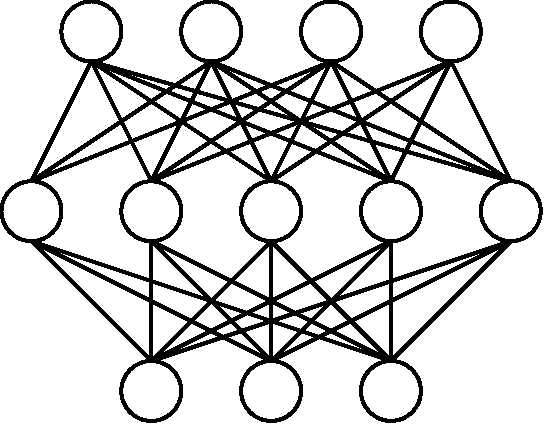
\includegraphics[scale=0.75]{fig/nn-blank.pdf}
			\end{center}
			\caption{A schematic representation of a deep neural network with an input layer, one hidden layer, and an output layer.}
			\label{fig:nn-blank}
		\end{figure}
		\par One big advantage to using a neural network is the ability of the neural network to output multiple values. Instead of the neural network taking state-action pairs and output scalar values, they can instead take states as input and produce vectors of $Q$ values corresponding to the quality of each action in that state. This is a much more efficient approach. We call this network the \kword{deep $Q$-network} (DQN). See figure \ref{fig:q-network-state-to-many-actions} for a schematic.
		\begin{figure}[ht]
			\begin{center}
				\textbf{$Q$-Network} \\
			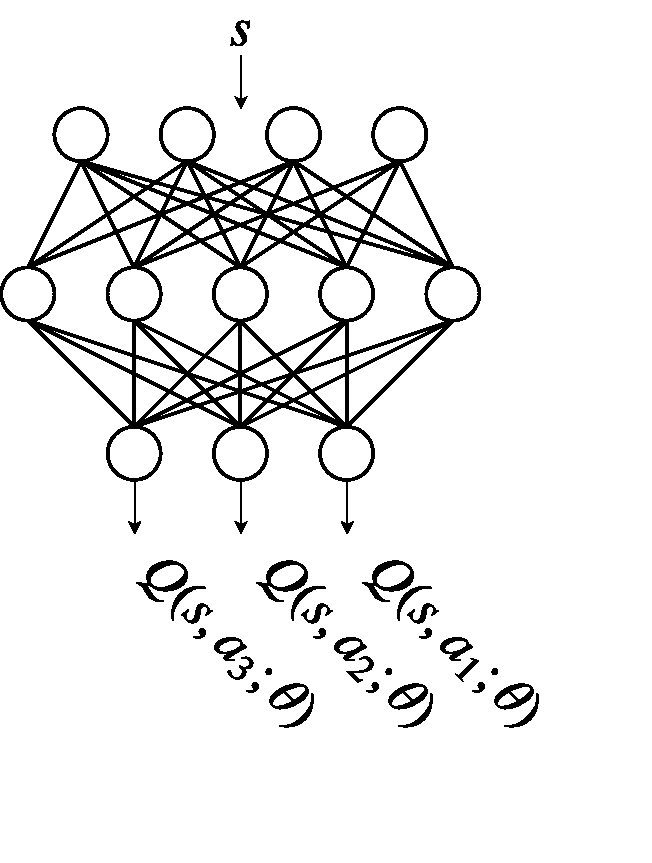
\includegraphics[scale=0.75]{fig/q-network-state-to-many-actions.pdf}
			\end{center}
			\caption{A $Q$-network. The state is a 4-dimensional vector and there are 3 discrete actions available. The network takes a state $s_t$ as a parameter and for each action $a$ predicts the quality $Q_\theta (s_t,a_t)$ of that action.}
			\label{fig:q-network-state-to-many-actions}
		\end{figure}
		\par Neural networks need to be differentiable so that we can use the optimization technique of \kword{gradient descent} to train it. Typically a neural network is specified abstractly as a set of parameters $\theta$ that determine the output of the network given the input. Then we represent $Q$ as a function parametrized by $\theta$: $Q_\theta$. We define a loss $L(\theta)$ for the network that we want to minimize. Gradient descent works by taking the gradient of $L$ with respect to $\theta$ and taking a small step in the direction opposite the gradient (`down' the gradient, i.e., gradient descent). This is the basic formulation; several modern extensions of gradient descent exist that improve training of neural networks, the details of which we will not cover in this thesis.
		\par Consider the $Q$-learning update rule (\ref{eqn:q_update_rule}). When $Q(s_t, a_t)$ is exactly equal to the TD target, there is no update. Noticing this, we might consider the loss of our neural network to be 0 when the value for $Q(s_t, a_t)$ is equal to $r_t + \gamma \max_{a_{t+1}} Q(s_{t+1}, a_{t+1})$. This is exactly the framework of a regression problem. We can then define the loss to be the squared error between the two:
		\begin{equation}
			\label{eqn:q_loss_no_target_network}
			L(\theta) = \mathbb{E}_{a_t \sim \pi}[(y_i - Q_\theta(s_t, a_t))^2]
		\end{equation}
		where the TD target is $y_i$:
		\begin{equation}
			\label{eqn:y_i_no_target_network}
			y_i = \mathbb{E}_{a_{t+1} \sim \pi} \left[ r_t + \gamma \max_{a_{t+1}}Q_\theta(s_{t+1}, a_{t+1}) \big\vert s_t, a_t \right]
		\end{equation}
		\par Training the neural network would consist of the following sequence of events:
		\begin{enumerate}
			\item The agent in state $s_t$ calculates $Q_\theta (s_t, a_t)$ using network parameters $\theta$ for each possible $a_t$. Using the greedy policy, it selects the action $a_t$ that maximizes $Q_\theta (s_t, a_t)$.
			\item As a result of choosing this action, the state transitions to state $s_{t+1}$. The agent recieves a reward $r_t$ as a result.
			\item The agent is now in state $s_{t+1}$ calculates $Q_\theta(s_{t+1}, a_{t+1})$ using network parameters $\theta$ for each possible $a_{t+1}$. The maximal value of $Q_\theta (s_{t+1}, a_{t+1})$ is chosen.
			\item The network is trained to minimize the loss, with $Q_\theta (s_t, a_t)$ being the prediction of the network, and with $y_i$ being the reward for transitioning and the discounted maximal $Q$ value for state $s_{t+1}$ determined in step $4$ (i.e., $r_t + \gamma \max_{a_{t+1}}Q_\theta (s_{t+1}, a_{t+1}))$.
		\end{enumerate}
		See figure \ref{fig:state-transition-q-learning-loss} for a diagrammatic representation.

		\par To perform any variation of gradient descent requires defining the gradient of the loss function. In this case, we can just apply the chain rule to (\ref{eqn:q_loss_no_target_network}). If we treat the TD target $y_i$ as a constant (which is appropriate), we get a rather simple expression for the gradient:
		\begin{equation}
			\label{eqn:q-learning-gradient-no-target}
			\nabla_\theta L(\theta) = \mathbb{E}_{a \sim \pi} \left[ 2(y_i - Q_\theta (s,a)) \nabla_\theta Q_\theta (s,a) \right]
		\end{equation}
		and to update the the network parameters, we simply use \kword{stochastic gradient descent}:
		\begin{equation}
			\label{eqn:stochastic-gradient-descent}
				\theta \gets \theta + \frac{1}{2} \alpha \nabla_\theta L(\theta)
		\end{equation}
		where $\alpha$ is the learning rate.

		\begin{figure}[ht]
			\begin{center}
			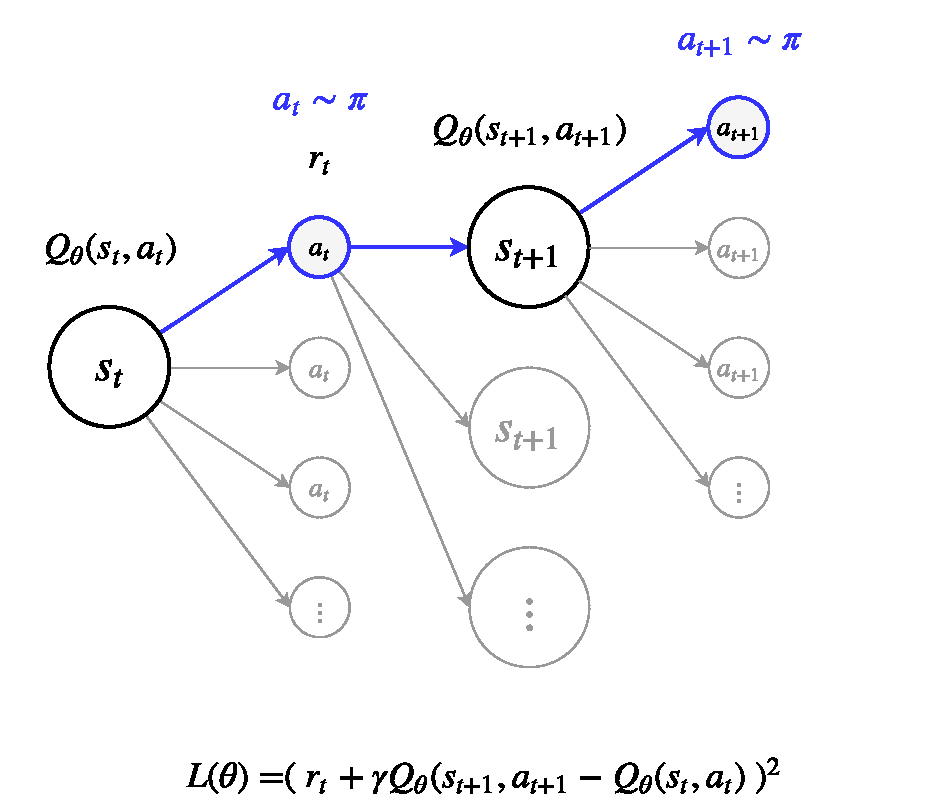
\includegraphics[scale=0.75]{fig/state-transition-q-learning-loss.pdf}
			\end{center}
			\caption{A diagram showing how $Q$-learning gathers data for training.}
			\label{fig:state-transition-q-learning-loss}
		\end{figure}
		\subsection{Target Networks}
		\par One may have realized that this network $\theta$ is trying to predict it own output. This kind of learning is unstable, meaning performance can quickly deteriorate (to even worse than random \cite{dqn}). One reason for this is that the neural network is differentiable. When we modify the parameters $\theta$ while training the network, we change the predictions for similar states to that which we just trained on. Since consecutive states tend to be similar, this can lead to an explosion in predicted values. Research has shown that training can be stabilized by using two networks: $\theta$ and $\theta_\text{targ}$. Instead of one set of parameters, we have two (i.e., we have two neural networks). We call the second network ($\theta_\text{targ}$) the \kword{target network}, and it uses the parameters from the $Q$-network that synchronize with the current $Q$-network every $n_\theta$ timesteps \cite{dqn}.
		\par We also define two policies:
		\begin{enumerate}
			\item $\pi$: The \kword{behaviour policy} that uses the $Q$-network ($Q_\theta (s_t,a_t)$) and is updated every time step.
			\item $\pi_\text{targ}$: The \kword{target policy} that uses the target network ($Q_{\theta_\text{targ}} (s_{t+1},a_{t+1})$) and is updated to match $\pi$ (i.e., $\theta_\text{targ}$ is updated to match $\theta$) every $n_\theta$ timesteps.
		\end{enumerate}
		Since the kind of predictions made by the target network $\theta_\text{targ}$ are static for $n_\theta$ timesteps, training becomes stabilized.
		\par As a result, we get a new formulation of (\ref{eqn:q_loss_no_target_network}):
		\begin{equation}
				\label{eqn:q_loss_target_network}
				L(\theta) = \mathbb{E}_{a \sim \pi} \left[ (y_i - Q_\theta(s_t,a_t))^2 \right]
		\end{equation}
		where the TD target is $y_i$:
		\begin{equation}
			\label{eqn:y_i_target_network}
			y_i = \mathbb{E}_{a_{t+1} \sim \pi_\text{targ}} \left[ r_t + \gamma \max_{a_{t+1}}Q_{\theta_\text{targ}}(s_{t+1}, a_{t+1}) \big\vert s_t, a_t \right]
		\end{equation}
		See figure \ref{fig:state-transition-q-learning-loss-target-networks} for a diagrammatic representation.
		\begin{figure}[ht]
			\begin{center}
			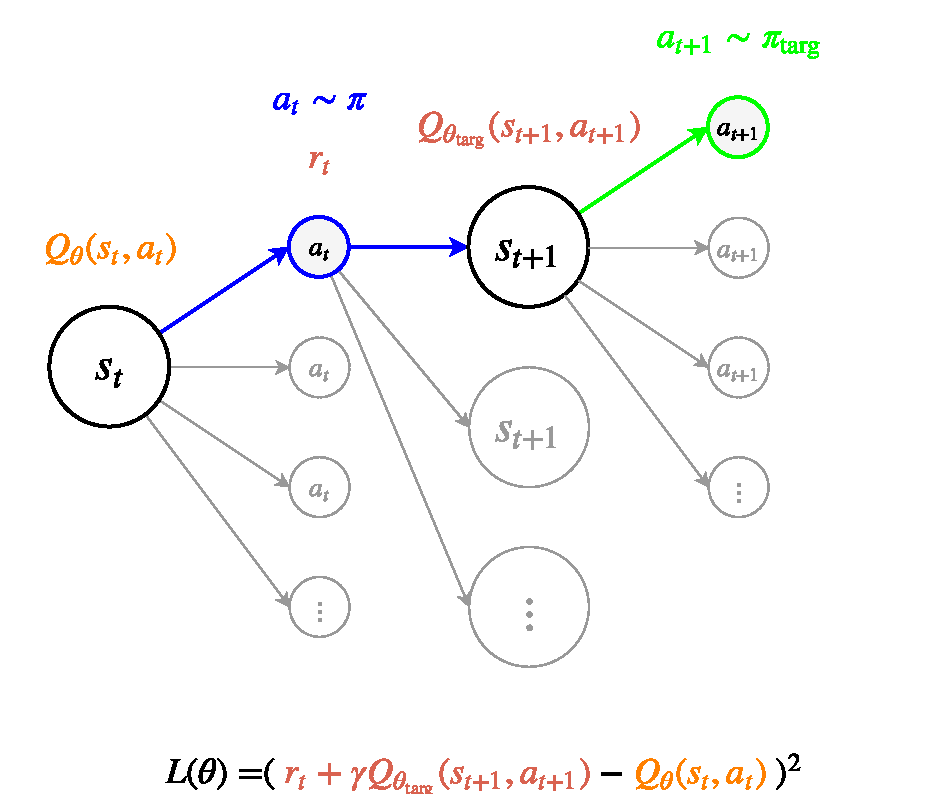
\includegraphics[scale=0.75]{fig/state-transition-q-learning-loss-target-networks.pdf}
			\end{center}
			\caption{A diagram showing how $Q$-learning gathers data for training using the target network and behaviour network.}
			\label{fig:state-transition-q-learning-loss-target-networks}
		\end{figure}

		\subsection{Exploration-Exploitation}
		\par One major problem in reinforcement learning is determining the optimal balance between \kword{exploration} and \kword{exploitation}. Exploitation refers to an agent's tendency to choose actions that it thinks are best for it at any given time. This is the case with our greedy behaviour policy $\pi$. This comes at the cost of potentially not exploring new states. For the neural network to well approximate the $Q$ function, it needs to have exposure to as much of $\mc{S}$ as possible.
		\par The epsilon-greedy strategy can be used to improve exploration. When using an epsilon-greedy strategy, we select a constant $0 \leq \epsilon \leq 1$ that chooses an action either randomly or according to $\pi$ by comparing a random number $p \sim \mc{U}(0,1)$ to $\epsilon$; if $p < \epsilon$ we choose a random action. Otherwise, we choose an action according to $\pi$.
		\par There are various strategies one can use for $\epsilon$-greedy policies. One example is to choose some initial value $\epsilon_i$ and some final value $\epsilon_f$, and a number of iterations $n_\epsilon$ over which $\epsilon_i$ decays into $\epsilon_f$ so that initially exploration is high and exploitation is low; as the network learns, it becomes more deterministic as it learns to exploit known rewards and techniques. Another strategy for episodic environments is to choose $\epsilon$ empirically:
		$$\epsilon = \frac{1}{\sqrt{T+1}}$$
		where $T$ is the time horizon of the episode.

		\subsection{Experience Replay}
		\par When we update our $Q$-network, we do it after every state transition (i.e., we do it \kword{online}). Recall that we are using gradient descent to train the network parameters $\theta$. One problem with training online is that we get a biased, high variance estimate for the gradient. A better approach would involve taking the mean gradient estimate of the loss over many pairs of $Q_\theta(s,a)$ and TD targets. Furthermore, by training the network only on the most recent state transition, we are only making the network better at predicting the most recent TD target. This can undo some of the progress made training the network on earlier transitions. This problem is known as \kword{catastrophic forgetting} \cite{dqn}.
		\par We can reduce the noise and bias in our gradient estimates by including an \kword{experience replay buffer} $\mc{D}$ that stores transitions
		$$\langle s_t, a_t, r_t, s_{t+1} \rangle$$
		Note that we do not need to store $a_{t+1}$ since our network will choose $a_{t+1}$ based on $\pi$ anyways. We then train the network by taking batches of transitions from $\mc{D}$. For each transition, we use the $Q$-network to predict $Q_\theta (s_t,a_t)$ and to consequently choose an action $a_t \sim \pi$, and we use the target network to predict $Q_{\theta_\text{targ}}(s_{t+1},a_{t+1})$ and to consequently choose an action $a_{t+1} \sim \pi_\text{targ}$. Over all transitions in the batch, we calculate the gradient of the loss $L(\theta)$. We take the average of these gradients and update the network parameters. \cite{dqn} showed that stability in learning is essential to good performance, and using an experience replay buffer helps with this.
		\subsection{Double $Q$-Learning}
		\par In the target network formulation of deep $Q$-learning, we use the target network to compute $Q_{\theta_\text{targ}}(s_{t+1}, a_{t+1})$. We use $\pi_\text{targ}$ to greedily choose an action $a_{t+1}$ as a result of this calculation. Thus, computing the quality of an action and choosing an action is tightly coupled. In double $Q$-learning, we decouple these \cite{ddqn}.
		\par We choose an action $a_{t+1}$ based on the current behaviour policy $\pi$ (that is, we calculate $Q_\theta(s_{t+1},a_{t+1})$ and select greedily from the results). We then use this $a_{t+1}$ to calculate $y_i$ (that is, we use $a_{t+1}$ to calculate $Q_{\theta_\text{targ}}(s_{t+1}, a_{t+1})$). As a result, we can rewrite our TD target $y_i$:
		\begin{equation}
			\label{eqn:y_i_double}
		y_i = \mathbb{E}_{a_{t+1} \sim \pi_\text{targ}} \left[ r_t + \gamma Q_{\theta_\text{targ}}(s_{t+1}, \arg \max_{a_{t+1}} Q_\theta (s_{t+1}, a_{t+1})) \big\vert s_t, a_t \right]
		\end{equation}
		See figure \ref{fig:state-transition-q-learning-loss-double} for a diagrammatic representation.
		\begin{figure}[ht]
			\begin{center}
			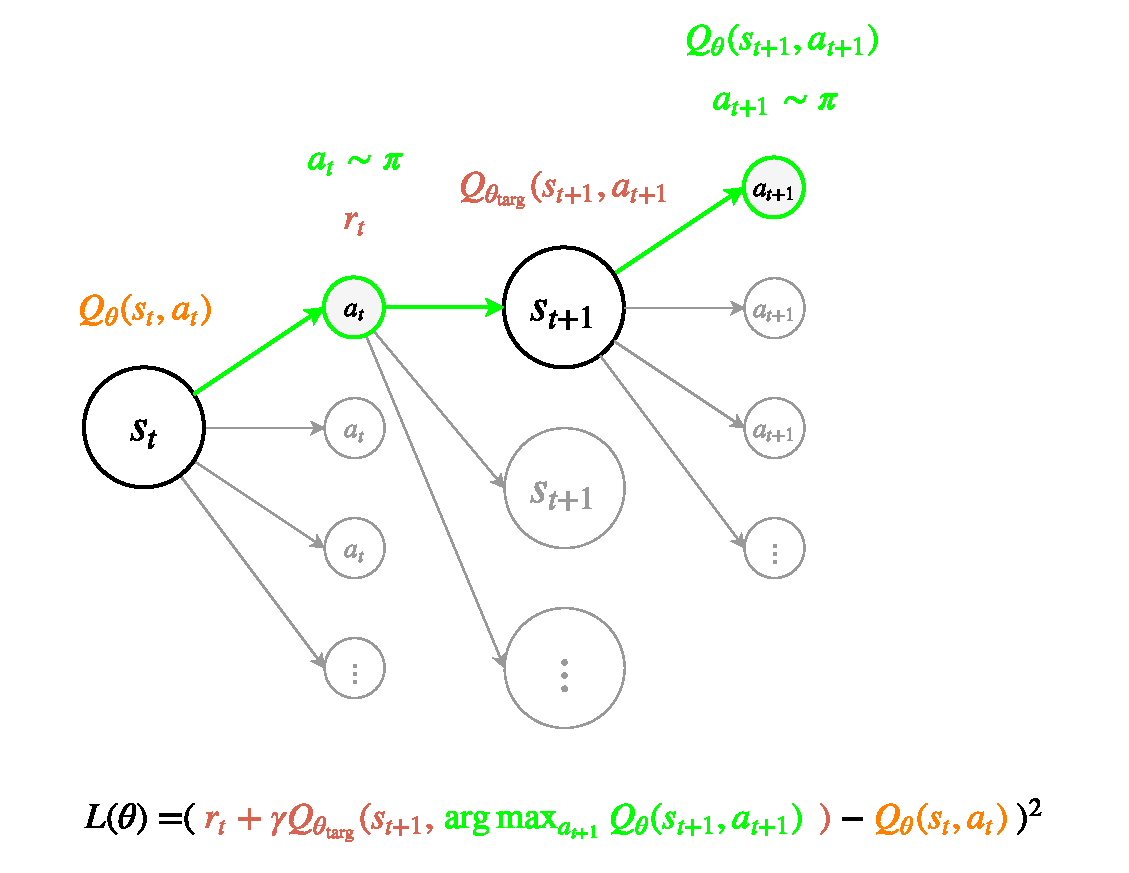
\includegraphics[scale=0.75]{fig/state-transition-q-learning-loss-double.pdf}
		\end{center}
			\caption{A diagram showing how $Q$-learning gathers data for training using double $Q$-learning.}
			\label{fig:state-transition-q-learning-loss-double}
		\end{figure}

		\newpage
		\section{Policy Gradients}
		\label{sec:policy-gradients}
		\par In $Q$-learning, we have a policy $\pi$ that is simply a greedy (or $\epsilon$-greedy) strategy. While this can be effective in problems with small (discrete) action spaces, we may face problems with large (or continuous) action spaces. We can circumvent this by instead directly trying to model $\pi$. We can parametrize the policy using some parameters $\theta$ to produce a distribution over actions:
		\begin{equation}
			\label{eqn:policy-as-distribution}
			\pi_\theta(a_t \big\vert s_t) = \mathbb{P}\left[ a_t \big\vert s_t; \theta \right]
		\end{equation}
		\par Modelling the policy directly has an additional advantage over the greedy policy from $Q$-learning, which is that it can learn a \kword{stochastic policy}. We have the option of picking an action stochastically over the distribution $\pi$.
		\par Consider some objective function $J$ that we want to maximize using our policy (and consequently $J$ is a function of $\theta$). An obvious choice would be the return given the policy $\pi_\theta$. There are three possible objectives:
		\begin{itemize}
			\item For episodic environments (i.e., with a finite time horizon $T$) we just consider the value of the starting state $s_0$.
			\begin{equation}
				\label{eqn:j-1-episodic}
				J_1(\theta) = V^{\pi_\theta}(s_0) = \mathbb{E}_{\pi_\theta} \left[ G_0 \right]
			\end{equation}

			\item For continuing environments, we can consider the average value over all states:
			\begin{equation}
				\label{eqn:j-1-average-value}
				J_{\text{av}V}(\theta) = \sum_{s \in \mc{S}} d^{\pi_\theta}(s) V^{\pi_\theta}(s)
			\end{equation}
			where $d^{\pi_\theta}(s)$ is the distribution of states over the policy $\pi_\theta$.
			\item For continuing environments, we can also consider the average reward per time step:
			\begin{equation}
				\label{eqn:j-1-average-reward}
				J_{\text{av}R}(\theta) = \sum_{s \in \mc{S}} d^{\pi_\theta}(s) \sum_{a \in \mc{A}} \pi_\theta (s, a) \mc{R}(s,a)
			\end{equation}
		\end{itemize}

		Consider an MDP with a single step (i.e., $T=1$). Then the objective function is just the expected reward for that single step. Evaluating this expectation yields the formula for average reward per timestep for one timestep, where the distribution of states over the policy is just the distribution of the MDP:
		\begin{align}
			\label{eqn:j-1-step-MDP}
			J(\theta) &= \mathbb{E}_{\pi_\theta} \left[ r \right] \\
			  				&=\sum_{s \in \mc{S}} d(s) \sum_{a \in \mc{A}} \pi_\theta (s, a) \mc{R}(s,a) \nonumber
		\end{align}
		How should we update the policy parameters $\theta$ so as to maximize this reward? A simple approach would be to use \kword{gradient ascent}, where we compute the gradient of the objective function with respect to our policy parameters $\theta$ and add this gradient vector to our parameters. Over time, then, we learn parameters $\theta$ that maximize $J(\theta)$ (unlike in $Q$-learning, where we use gradient descent to minimize $L(\theta)$).
		\begin{equation}
			\label{eqn:gradient-ascent}
			\theta \gets \theta + \alpha \nabla_\theta J(\theta)
		\end{equation}
		where for the single-step MDP the gradient is:
		\begin{equation}
			\label{eqn:gradient-of-j}
			\nabla_\theta J(\theta) = \sum_{s \in \mc{S}} d(s) \sum_{a \in \mc{A}} \nabla_\theta \pi_\theta (s, a) \mc{R}(s,a)
		\end{equation}
		This form almost looks like our original expectation in (\ref{eqn:j-1-step-MDP}) except that it is missing the probability distribution over actions. We can reintroduce it by multiplying and dividing by $\pi_\theta(s,a)$ (with the exception that the policy must not be 0 which is satisfied almost everywhere).
		\begin{align}
			\label{eqn:gradient-ascent-mult-div}
			\nabla_\theta J(\theta) &= \sum_{s \in \mc{S}} d(s) \sum_{a \in \mc{A}} \pi_\theta (s, a) \frac{\nabla_\theta \pi_\theta (s, a)}{\pi_\theta (s, a)} \mc{R}(s,a) \\
			&= \mathbb{E}_{\pi_\theta} \left[ \frac{\nabla_\theta \pi_\theta (s, a)}{\pi_\theta (s, a)} r \right]
		\end{align}
		This expression for the gradient is extremely intuitive. The top is a vector in parameter space that would move $\theta$ in the direction that increases the probability of choosing action $a$ in state $s$. However, this could lead to a feedback loop where we just continually take the most likely action, so to counteract this, we divide by the probability of taking this action. Finally, we scale by the reward; the higher the reward, we more we want to take this action. We can use the following identity to make the expresson even simpler:
		\begin{equation}
			\label{eqn:log-identity}
			\frac{\nabla_\theta \pi_\theta (s, a)}{\pi_\theta (s, a)} = \nabla_\theta \log \pi_\theta (s, a)
		\end{equation}
		For multi-step MDPs, we can replace the reward $r$ for a single time step with the long-term quality $Q^{\pi_\theta}(s,a)$, since we are taking the expectation over all states and actions according to our policy $\pi_\theta$. Combining this with (\ref{eqn:log-identity}) yields \kword{the policy gradient theorem}:
		\begin{equation}
			\label{eqn:the-policy-gradient-theorem}
			\nabla_\theta J(\theta) = \mathbb{E}_{\pi_\theta} \left[ \nabla_\theta \log \pi_\theta (s, a) Q^{\pi_\theta}(s,a) \right]
		\end{equation}
		\subsection{REINFORCE}
		\par Since the policy gradient theorem gives the gradient of the objective function as an expectation, we can sample this expectation to get an estimate for the gradient. Consider an episodic environment that terminates after $T$ time steps. At the end, we have a return $G_t$ for each time step. We can use the return for each time step as an unbiased estimate for $Q^{\pi_\theta}(s,a)$. For each timestep $t$ we can just update the policy parameters according to a modified version of (\ref{eqn:gradient-ascent}):
		\begin{equation}
			\label{eqn:reinforce-gradient-ascent}
			\theta \gets \theta + \alpha \nabla_\theta \log \pi_\theta(s_t,a_t)G_t
		\end{equation}
		\par This algorithm is known as the \kword{REINFORCE} algorithm \cite{rl}. The strategy of sampling complete episodes to gather information before making updates is called \kword{Monte Carlo policy gradient control}, where `Monte Carlo' means taking samples to approximate an expectation.
		\subsection{Actor-Critic (AC)}
		\par REINFORCE has a few problems:
		\begin{enumerate}
			\item Monte Carlo approximation is slow and subject to high variance.
			\item We need to know the final return before making any updates.
			\item It relies on episodic environments; what about continuing ones (i.e., $T = \infty$)?
		\end{enumerate}
		\par One approach would be to estimate $Q^{\pi_\theta}$ using a function approximator parametrized by parameters $\phi$. Then at each time step, we perform gradient ascent using not the true return, but a biased estimate $Q_\phi(s,a)$.
		\begin{equation}
			\label{eqn:action-value-critic-appx-equal}
			Q_\phi(s,a) \approx Q^{\pi_\theta}(s,a)
		\end{equation}
		If we carefully choose our function approximator $\phi$ then we can ensure that the replacing $ Q^{\pi_\theta}(s,a)$ with $Q_\phi(s,a)$ yields the exact same gradient as in the policy gradient theorem. We need to satisfy two conditions:
		\begin{enumerate}
			\item The function approximator must be \kword{compatible} to the policy
			\begin{equation}
				\label{eqn:compatible}
				\nabla_\phi Q_\phi(s,a) = \nabla_\theta \log \pi_\theta (s,a)
			\end{equation}
			\item The parameters must minimize the mean-squared error between $Q^{\pi_\theta}(s,a)$ and $Q_\phi(s,a)$:
			\begin{equation}
				\label{eqn:minimize-mean-squared-error}
				\varepsilon = \mathbb{E}_{\pi_\theta} \left[ (Q_\phi(s,a) - Q^{\pi_\theta}(s,a))^2 \right]
			\end{equation}
		\end{enumerate}
		Then we can prove that the gradient remains unchanged. Since $\phi$ is chosen so as to minimize $\varepsilon$, we can state the following:
		\begin{align}
			\label{eqn:proof-of-exactness}
			\begin{split}
				\nabla_\phi \varepsilon &= 0 \\
				\mathbb{E}_{\pi_\theta} \left[ (Q_\phi(s,a) - Q^{\pi_\theta}(s,a)) \nabla_\phi Q_\phi(s,a) \right] &= 0 \text{ by the chain rule} \\
				\mathbb{E}_{\pi_\theta} \left[ (Q_\phi(s,a) - Q^{\pi_\theta}(s,a)) \nabla_\theta \log \pi_\theta (s,a) \right] &= 0 \text{ by compatability} \\
				\mathbb{E}_{\pi_\theta} \left[ Q_\phi(s,a) \nabla_\theta \log \pi_\theta (s,a) \right] &= \mathbb{E}_{\pi_\theta} \left[ Q^{\pi_\theta}(s,a) \nabla_\theta \log \pi_\theta (s,a) \right]
			\end{split}
		\end{align}
		Therefore we can substitute $Q_\phi(s,a)$ in for $Q^{\pi_\theta}(s,a)$ in the policy gradient theorem:
		\begin{equation}
			\label{eqn:policy-gradient-theorem-with-approximator}
			\nabla_\theta J(\theta) = \mathbb{E}_{\pi_\theta} \left[ \nabla_\theta \log \pi_\theta (s, a) Q_\phi(s,a) \right]
		\end{equation}
		\par We maintain two sets of parameters. One, $\theta$, is used to drive the policy $\pi_\theta$ and is used to select the actions of the agent. The second, $\phi$, is only used to estimate the quality of the actions taken by the policy in different states (and consequently suggests to the policy how to change in order to improve, as we can see by the $Q_\phi(s,a)$ term in the policy gradient). The function approximator for the policy is called the \kword{actor} and the function approximator for the quality is called the \kword{critic}.
		\par We have two sets of parameters to manage and optimize now. The first, $\theta$, can be trained using gradient ascent and the policy gradient theorem in (\ref{eqn:policy-gradient-theorem-with-approximator}), which can be done online (i.e., every time step). The second, $\phi$, can be trained exactly as in earlier sections using, for example, deep $Q$ learning.
		\par Actor-critic models are more \kword{data efficient} than methods like REINFORCE because they require less training examples in general to reach optimal performance.

		\subsection{Advantage Actor-Critic (A2C)}
		\par One issue with actor-critic models is that the quality $Q_\phi(s,a)$ can have high variance. One way to avoid this might be to consider subtracting some baseline $b(s)$ from the quality. We can show that making this change doesn't impact the expectation of the policy gradient theorem:
		\begin{align}
			\label{eqn:proof-of-baseline-no-differece}
			\begin{split}
				\nabla_\theta J(\theta) &= \mathbb{E}_{\pi_\theta} \left[ \nabla_\theta \log \pi_\theta (s, a) (Q_\phi(s,a) - b(s)) \right]\\
				&= \mathbb{E}_{\pi_\theta} \left[ \nabla_\theta \log \pi_\theta (s, a)Q_\phi(s,a) \right] - \mathbb{E}_{\pi_\theta} \left[ \nabla_\theta \log \pi_\theta (s, a) b(s) \right] \\
				\mathbb{E}_{\pi_\theta} \left[ \nabla_\theta \log \pi_\theta (s, a) b(s) \right] &= \sum_{s \in \mc{S}} d^{\pi_\theta}(s) \sum_{a \in \mc{A}} \nabla_\theta \pi_\theta (s, a) b(s) \\
				&= \sum_{s \in \mc{S}} d^{\pi_\theta}(s) b(s) \nabla_\theta \sum_{a \in \mc{A}}  \pi_\theta (s, a) \\
				&= \sum_{s \in \mc{S}} d^{\pi_\theta}(s) b(s) \nabla_\theta 1 \\
				&= 0 \\
				\nabla_\theta J(\theta) &= \mathbb{E}_{\pi_\theta} \left[ \nabla_\theta \log \pi_\theta (s, a)Q_\phi(s,a) \right] - 0\\
				\nabla_\theta J(\theta) &= \mathbb{E}_{\pi_\theta} \left[ \nabla_\theta \log \pi_\theta (s, a) (Q_\phi(s,a) - b(s)) \right] \\ &= \mathbb{E}_{\pi_\theta} \left[ \nabla_\theta \log \pi_\theta (s, a) Q_\phi(s,a) \right]
			\end{split}
		\end{align}
		So the expectation does not change even when including a baseline. Of couse we are now faced with an obvious question: what function should we use for the baseline?
		\par Consider the difference between $Q^{\pi_\theta}(s,a)$ and $V^{\pi_\theta}(s)$. $Q^{\pi_\theta}(s,a)$ tells us the expected return of taking an action $a$ in state $s$, then following the policy $\pi_\theta$. On the other hand, $V^{\pi_\theta}(s)$ tells us the expected return of following the policy $\pi_\theta$ starting in state $s$. Then there is some advantage to taking a specific action $a$ in state $s$ compared to just following the policy $\pi_\theta$ in state $s$, which we call the \kword{advantage} $A^{\pi_\theta}(s,a)$.
		\begin{align}
			\label{eqn:advantage}
				Q^{\pi_\theta}(s,a) &= V^{\pi_\theta}(s) + A^{\pi_\theta}(s,a) \\
				A^{\pi_\theta}(s,a)  &= Q^{\pi_\theta}(s,a) - V^{\pi_\theta}(s)
		\end{align}
		The advantage is exactly the form described in (\ref{eqn:proof-of-baseline-no-differece}). Thus, if we can estimate $A^{\pi_\theta}(s,a)$, we have a lower variance estimate for the gradient of the objective function.
		\begin{equation}
			\label{eqn:j-gradient-with-advantage}
			\nabla_\theta J(\theta) = \mathbb{E}_{\pi_\theta} \left[ \nabla_\theta \log \pi_\theta (s, a) A^{\pi_\theta}(s,a) \right]
		\end{equation}
		\par We are now faced with the challenge of estimating the advantage $A^{\pi_\theta}(s,a)$. We might consider using an approach similar to actor-critic, where insted of one set of parameters $\phi$ to predict $Q^{\pi_\theta}(s,a)$ we have two sets of parameters $\phi, \phi '$ where one predicts $Q^{\pi_\theta}(s,a)$ and the other predicts $V^{\pi_\theta}(s)$. It turns out that we can estimate the advantage using a single set of parameters.
		\par Let us denote the TD target error for the true value function $V^{\pi_\theta}(s_t)$ as $\delta_t^{\pi_\theta}$.
		\begin{equation}
			\label{eqn:td-target-error-true-v}
			\delta_t^{\pi_\theta} = r + \gamma V^{\pi_\theta}(s_{t+1}) - V^{\pi_\theta}(s_t)
		\end{equation}
		It turns out that this is an unbiased estimate of the advantage function:
		\begin{align}
			\begin{split}
				\mathbb{E}_{\pi_\theta} \left[ \delta_t^{\pi_\theta} \big\vert s_t, a_t \right] &= \mathbb{E}_{\pi_\theta} \left[ r + \gamma V^{\pi_\theta}(s_{t+1}) \big\vert s_t, a_t \right] - V^{\pi_\theta}(s) \\
				&= Q^{\pi_\theta}(s,a) - V^{\pi_\theta}(s)  \text{ by the definition of } Q^{\pi_\theta}(s,a) \\
				&= A^{\pi_\theta}(s,a )
			\end{split}
		\end{align}
		Then we can directly substitute $A^{\pi_\theta}(s,a)$ for $\delta_t^{\pi_\theta}$ in (\ref{eqn:j-gradient-with-advantage}):
		\begin{equation}
			\label{eqn:j-gradient-with-delta}
			\nabla_\theta J(\theta) = \mathbb{E}_{\pi_\theta} \left[ \nabla_\theta \log \pi_\theta (s, a) \delta_t^{\pi_\theta} \right]
		\end{equation}
		\par One way we can interpret this is that $\delta_t^{\pi_\theta}$ measures our error in how good we think the world is. If it is positive, then we were doing better than expected and should increase the probability of these actions in the future. If it is negative, then we were doing worse than expected and should decrease the probability of these actions in the future. What this means is that in practice, we only need one set of parameters for predicting $V^{\pi_\theta}(s)$, which we can denote $V_\phi(s)$, in order to calculate the TD error, which we can denote $\delta_t(\phi)$.
		\par This is really beneficial and practical for implementations of actor-critic, since we can train the critic by minimizing $\delta_t(\phi)^2$ (the squared error, as in (\ref{eqn:q_loss_no_target_network})) using gradient descent, and we can reuse $\delta_t(\phi)$ when training our actor using the policy gradient theorem and gradient ascent.
		\subsection{Generalized Advantage Estimation (GAE)}
		\par So far, we have seen several forms of the policy gradient equation. They are all of the following form:
		\begin{equation}
			\label{eqn:generalized-gradient}
			g = \mathbb{E}_{\pi_\theta} \left[ \sum_{t=0}^\infty \Psi_t \nabla_\theta \log \pi_\theta(a_t \big\vert s_t) \right]
		\end{equation}
		where $g$ is notational shorthand for the gradient of the objective function $\nabla_\theta J(\theta)$, and where $\Psi_t$ is one of any of the following:
		\begin{align}
			\label{eqn:psi-options}
			\begin{split}
				R_t &= \sum_{k=t}^\infty r_k\\
				G_t &= \sum_{k=t}^\infty \gamma^{k-t}r_k
			\end{split}
			\begin{split}
				Q^{\pi_\theta}(s_t, a_t) \\
				A^{\pi_\theta}(s_t, a_t) &= Q^{\pi_\theta}(s_t, a_t) - V^{\pi_\theta}(s_t) \\
				\delta_t^{\pi_\theta} &= r_t + V^{\pi_\theta}(s_{t+1}) - V^{\pi_\theta}(s_t)
			\end{split}
		\end{align}
		We consider the undiscounted return versions of the value, action-value, and advantage:
		\begin{align*}
					V^{\pi_\theta}(s_t) &= \mathbb{E}_{\pi_\theta} \left[ R_t \big\vert s_t \right] \\
					Q^{\pi_\theta}(s_t, a_t) &= \mathbb{E}_{\pi_\theta} \left[ R_t \big\vert s_t, a_t \right] \\
					A^{\pi_\theta}(s_t, a_t) &= Q^{\pi_\theta}(s_t, a_t) - V^{\pi_\theta}(s_t)
		\end{align*}
		And specify $\gamma$ as a parameter:
		\begin{align*}
					V^{\pi_\theta, \gamma}(s_t) &= \mathbb{E}_{\pi_\theta} \left[ G_t \big\vert s_t \right] \\
					Q^{\pi_\theta, \gamma}(s_t, a_t) &= \mathbb{E}_{\pi_\theta} \left[ G_t \big\vert s_t, a_t \right] \\
					A^{\pi_\theta, \gamma}(s_t, a_t) &= Q^{\pi_\theta, \gamma}(s_t, a_t) - V^{\pi_\theta \gamma}(s_t)
		\end{align*}
		Then we can use the advantage to define a policy gradient with $\gamma$ as a parameter.
		\begin{equation}
			\label{eqn:generalized-advantage}
			g^\gamma = \mathbb{E}_{\pi_\theta} \left[ \sum_{t=0}^\infty A^{\pi_\theta, \gamma} \nabla_\theta \log \pi_\theta(a_t \big\vert s_t) \right]
		\end{equation}
		\par Generalized advantage estimation (GAE) is an approach that deals with trying to balance between bias and variance for estimating the advantage $A^{\pi_\theta, \gamma}$, which we will call $\hat{A}$. In order to estimate the gradient in (\ref{eqn:generalized-advantage}), we take samples from the environment.
		\begin{equation}
			\label{eqn:gradient-estimator}
			\hat{g}^\gamma = \frac{1}{N} \sum_{n=1}^N \sum_{t=0}^\infty \hat{A}^n_t \nabla_\theta \log \pi_\theta(a_t \big\vert s_t)
		\end{equation}
		\par Recall that the TD-difference $\delta_t^{\pi_\theta}$ is an unbiased estimate of $A^{\pi_\theta, \gamma}$. Let us denote $\hat{A}_t^{(k)}$ to be the sum of $k$ terms of $\delta_t^{\pi_\theta}$.
		\begin{align*}
			\hat{A}_t^{(1)} &= \delta_t^{\pi_\theta} &&= -V_\phi(s_t) + r_t + \gamma V_\phi(s_{t+1}) \\
			\hat{A}_t^{(2)} &= \delta_t^{\pi_\theta} + \gamma \delta_{t+1}^{\pi_\theta} &&= -V_\phi(s_t) + r_t + \gamma r_{t+1} +  \gamma^2 V_\phi(s_{t+2}) \\
			\hat{A}_t^{(3)} &= \delta_t^{\pi_\theta} + \gamma \delta_{t+1}^{\pi_\theta} + \gamma^2 \delta_{t+2}^{\pi_\theta} &&= -V_\phi(s_t) + r_t + \gamma r_{t+1} + \gamma^2 r_{t+2} \gamma^3 V_\phi(s_{t+3}) \\
			\vdots &&& \vdots \\
			\hat{A}_t^{(k)} &= \sum_{i=0}^k \gamma^i \delta_{t+i}^{\pi_\theta} &&= -V_\phi(s_t) + r_t + \gamma r_{t+1} + \dots + \gamma^{k-1} r_{t+k-1} +  \gamma^k V_\phi(s_{t+k}) \\
		\end{align*}
		where $\hat{A}_t^{(k)}$ is essentially a $k$-term estimate of the return, minus a baseline term $-V^{\pi_\theta}(s_t)$. In general, the bias becomes smaller as $k \to \infty$ since $\gamma^k V(s_{t+k})$ becomes more heavily discounted as $k$ increases. Furthermore, as previously established, subtracting a baseline does not impact the expectation. Taking the limit $k \to \infty$ yields
		\begin{equation}
			\hat{A}_t^{(\infty)} = \sum_{i=0}^\infty \gamma^i \delta_{t+i}^{\pi_\theta} = -V_\phi(s_t) + \sum_{i=0}^\infty \gamma^i r_{t+i}
		\end{equation}
		which ends up just being the empirical returns minus a the value-function baseline.
		\par The generalized advantage estimator $\text{GAE}(\gamma, \lambda)$ is just an exponentially-weighted average of these $k$-step estimators:
		\begin{align*}
			\hat{A}_t^{\text{GAE}(\gamma, \lambda)} &= (1-\lambda)\left(\hat{A}_t^{(1)} + \lambda \hat{A}_t^{(2)} +  \lambda^2 \hat{A}_t^{(3)} + \dots \right) \\
			&= (1-\lambda)\left(\delta_{t}^{\pi_\theta} + \lambda (\delta_{t}^{\pi_\theta} + \gamma \delta_{t+1}^{\pi_\theta}) +  \lambda^2 (\delta_{t}^{\pi_\theta} + \gamma \delta_{t+1}^{\pi_\theta} + \gamma^2 \delta_{t+2}^{\pi_\theta}) + \dots \right) \\
			&= (1-\lambda) (\delta_{t}^{\pi_\theta}(1 + \lambda + \lambda^2 + \dots) + \gamma \delta_{t+1}^{\pi_\theta}(\lambda + \lambda^2 + \lambda^3 + \dots) + \\ & \quad \quad  \gamma^2\delta_{t+2}^{\pi_\theta}(\lambda^2 + \lambda^3 + \lambda^4 + \dots) + \dots ) \\
			&= (1-\lambda) \left(\delta_{t}^{\pi_\theta}\left(\frac{1}{1-\lambda}\right) + \gamma \delta_{t+1}^{\pi_\theta}\left(\frac{\lambda}{1-\lambda}\right) + \gamma^2 \delta_{t+2}^{\pi_\theta}\left(\frac{\lambda^2}{1-\lambda}\right) \right) \\
			&= \sum_{i=0}^\infty (\gamma \lambda)^i \delta_{t+i}^{\pi_\theta}
		\end{align*}
		\cite{gae} cites two special cases of GAE, which are achieved by setting $\gamma = 0$ and $\gamma=1$.
		\begin{align*}
			\text{GAE}(\gamma, 0): \hat{A}_t &= \delta_{t}^{\pi_\theta} &= r_t + \gamma V_\phi(s_{t+1}) - V_\phi(s_{t}) \\
			\text{GAE}(\gamma, 1): \hat{A}_t &= \sum_{i=0}^\infty \gamma^i \delta_{t+i}^{\pi_\theta} &= \sum_{i=0}^\infty \gamma^i r_{t+i} - V_\phi(s_{t}) \\
		\end{align*}
		\par Both $\gamma$ and $\lambda$ are parameters that contribute to the bias-variance tradeoff. $\gamma$ determines the scale of the value function $V^{\pi_\theta, \gamma}$ which does not depend on $\lambda$. Regardless of the accuracy of $V_\phi$, taking $\gamma < 1$ introduces a bias into the policy gradient estimate. On the other hand, taking $\lambda < 1$ introduces bias only when $V_\phi$ is inaccurate. Empirically, \cite{gae} find that the best value of $\lambda$ is much lower than the best value of $\gamma$.
		\par Using GAE, we can construct a biased estimator of $g^\gamma$:
		\begin{equation}
			\label{eqn:g-gamma-estimate}
			g^\gamma \approx \mathbb{E} \left[ \sum_{t=0}^\infty \nabla_\theta \log \pi_\theta (a_t \big\vert s_t) \hat{A}_t^{\text{GAE}(\gamma, \lambda)} \right] = \mathbb{E} \left[ \sum_{t=0}^\infty \nabla_\theta \log \pi_\theta (a_t \big\vert s_t) \sum_{i=0}^\infty (\gamma \lambda)^i \delta_{t+i}^{\pi_\theta} \right]
		\end{equation}
		where the equality holds when $\lambda = 1$.
		\subsection{Proximal Policy Optimization (PPO)}
		\par We next cover a relatively simple algorithm that performs at least as well as those listed above: \kword{proximal policy optimization} (PPO) \cite{ppo}.
		\par In PPO, our objective function is different than our expected return (or other variants mentioned above). Instead, we begin by considering a \kword{surrogate objective}, first described in a method called conservative policy iteration (CPI) \cite{ppo}:
		\begin{equation}
			\label{eqn:CPI}
			J^{\text{CPI}}(\theta) = \mathbb{E}_{\pi_\theta} \left[ \frac{\pi_\theta (a \vert s)}{\pi_{\theta_\text{old}}(a \vert s)}A^{\pi_\theta}(a, s) \right]
		\end{equation}
		In this case, we have some old policy parameters $\theta_\text{old}$ and some new policy parameters $\theta$. We calculate the ratio of the policies $\rho (\theta)$: \footnote{The authors of the original paper use $r(\theta)$ but we will use $\rho$ to avoid confusion.}
		\begin{equation}
			\label{eqn:ratio-of-policies}
			\rho(\theta) = \frac{\pi_\theta (a \vert s)}{\pi_{\theta_\text{old}}(a \vert s)}
		\end{equation}
		Which simplifies our notation a bit. Then our surrogate objective can be written as
		\begin{equation}
			\label{eqn:CPI-using-rho}
			J^{\text{CPI}}(\theta) = \mathbb{E}_{\pi_\theta} \left[ \rho(\theta) A^{\pi_\theta}(s,a) \right]
		\end{equation}
		The intuition here is that if we update our policy parameters, we want that update to make sense.
		\begin{itemize}
			\item If our advantage is positive and $\rho (\theta)$ is positive (i.e., we just made our action more likely) then we want to increase the likelihood of making this kind of update again in the future (i.e., updating from $\theta_\text{old}$ to $\theta$ was a good idea).
			\item If our advantage is negative and $\rho(\theta)$ is positive, then we want to decrease our likelihood of making this kind of update again in the future (i.e., updating from $\theta_\text{old}$ to $\theta$ was a bad idea).
			\item If our advantage is positive and $\rho(\theta)$ is negative, then we want to decrease our likelihood of making this kind of update again in the future.
			\item If our advantage is negative and $\rho(\theta)$ is negative, then we want to increase the likelihood of this kind of update again in the future.
		\end{itemize}
		\par The only problem with this surrogate objective is that it is unconstrained and could lead to destructive updates to the policy. While PPO in general is an entire family of algorithms proposed in \cite{ppo}, here we consider the \kword{clipped surrogate objective function}:
		\begin{equation}
			\label{eqn:clipped-objective-function}
			J^\text{CLIP}(\theta) = \mathbb{E}_{\pi_\theta} \left[ \min \left( \rho(\theta), \text{clip} (\rho(\theta), 1-\epsilon, 1+\epsilon) \right)  A^{\pi_\theta}(s,a) \right]
		\end{equation}
		Here, $\text{clip}(\rho(\theta), 1-\epsilon, 1+\epsilon)$ clips $\rho(\theta)$ into the range $[1-\epsilon, 1+\epsilon]$. By taking the minimum between $\rho(\theta)$ and the clipped version, we ensure that any updates to our policy are conservative and that $J^\text{CLIP}(\theta)$ is a lower bound for the unclipped objective.
		\par To elaborate on this, consider two cases:
		\begin{itemize}
			\item $A^{\pi_\theta}(s,a)$ is positive. Consider what happens as $\rho(\theta)$ changes from being below 1 to being above 1 (figure \ref{fig:clipped-objective-a-gtz}).
			\begin{figure}[ht]
				\begin{center}
				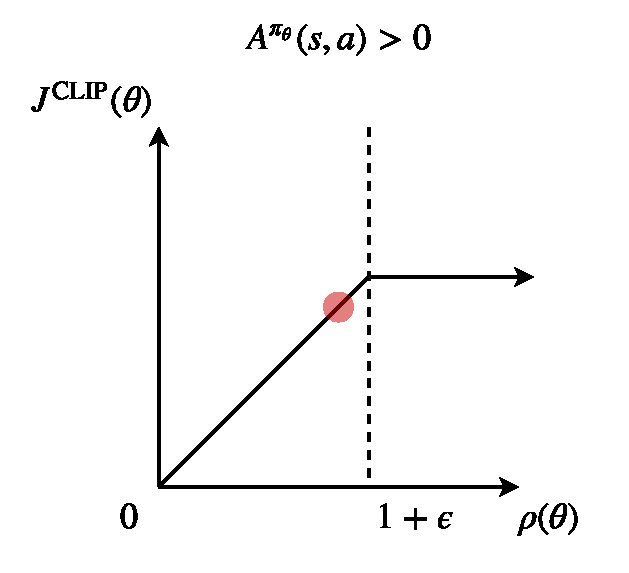
\includegraphics[scale=0.75]{fig/clipped-objective-a-gtz.pdf}
			\end{center}
				\caption{How the objective changes as $\rho(\theta)$ changes when $A^{\pi_\theta}(s,a) > 0$. Adapted from \cite{ppo}. The red dot indicates $\rho(\theta) = 1$.}
				\label{fig:clipped-objective-a-gtz}
			\end{figure}
			Once $\rho(\theta)$ increases beyond $1 + \epsilon$, there is no further increase in objective and the gradient is clipped to zero.
			\par In this case, the action was good ($A^{\pi_\theta}(a,s) > 0$).
			\begin{itemize}
				\item If the action became more probable ($\rho(\theta) > 1$) then we allow the gradient to improve the policy only a little bit, since too large of an optimistic gradient update can be destructive to the policy. Clipping helps control the magnitude of gradient updates.
				\item If the action became less probable ($\rho(\theta) < 1$) then we place no restriction on improving the policy (i.e., we are free to roll back the adjustment we just made). We only freely update the policy using the full gradient when we performed worse than expected.
			\end{itemize}
			\item $A^{\pi_\theta}(s,a)$ is negative. Consider what happens as $\rho(\theta)$ changes from being above 1 to being below 1 (figure \ref{fig:clipped-objective-a-ltz})
			\begin{figure}[ht]
				\begin{center}
				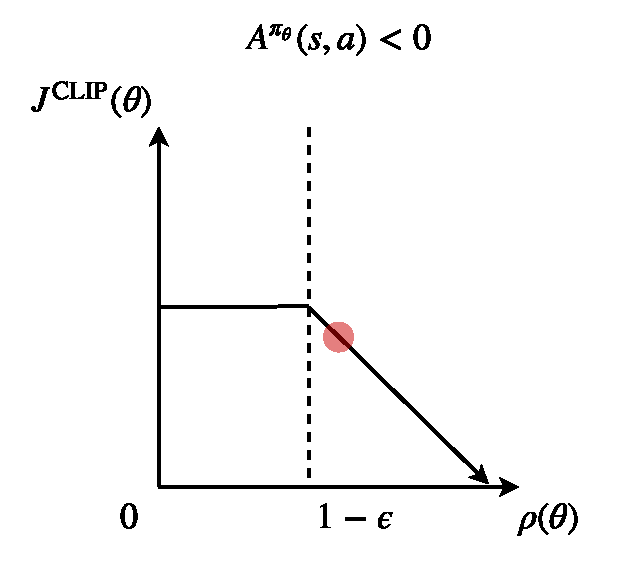
\includegraphics[scale=0.75]{fig/clipped-objective-a-ltz.pdf}
			\end{center}
				\caption{How the objective changes as $\rho(\theta)$ changes when $A^{\pi_\theta}(s,a) < 0$. Adapted from \cite{ppo}. The red dot indicates $\rho(\theta) = 1$.}
				\label{fig:clipped-objective-a-ltz}
			\end{figure}
			Once $\rho(\theta)$ decreases beyond $1 - \epsilon$, there is no further increase in objective and the gradient is clipped to zero.
			\par In this case, the action was bad ($A^{\pi_\theta}(a,s) < 0$).
			\begin{itemize}
				\item If the action became less probable ($\rho(\theta) < 1$) then we allow the gradient to improve the policy only a little bit, since too large of an optimistic gradient update can be destructive to the policy. Clipping helps control the magnitude of gradient updates.
				\item  If the action became more probable ($\rho(\theta) > 1$) then we place no restriction on improving the policy.
			\end{itemize}
		\end{itemize}

		\par In methods like actor-critic, it may be tempting to update the policy repeatedly on the same set of data to try to encourage quicker convergence to an optimum. The issue with this is that often such repeated updates are destructive. The main advantage of PPO is that we can train the policy by taking minibatches of transitions from an experience replay buffer $\mc{D}$ and perform gradient ascent over multiple epochs on this data without destroying the policy since our updates are conservative (and the gradient goes to 0 if the update is too large). This gives us a high amount of \kword{data efficiency}; we need less data to perform as well as methods like A2C (and so in a sense, PPO performs `better').

		\subsection{Deep Deterministic Policy Gradients (DDPG)}
		\par The last kind of policy gradient agent we will be interested in extends deep $Q$-learning to continuous action spaces. Recall that DQNs work for discrete action spaces only, since we use a greedy policy that selects the action with the highest predicted $Q$ value, and this requires outputting a predicted $Q$ value for every possible action. Consider a $n$-dimensional action space discretized into $\{-k,0, k \}$ for each dimension. Then discretizing the action space produces $3^n$ possible actions, which quickly becomes intractable for high-dimensional output spaces.
		\par We can describe an optimal action taken by the greedy policy described in (\ref{eqn:greedy_policy}):
		\begin{equation}
			\label{eqn:optimal-action}
			a_t^*(s_t) = \arg \max_{a_t} Q^*(s_t,a_t)
		\end{equation}
		to extend this to continuous action spaces, we simply define a deterministic policy $\mu: \mc{S} \to \mc{A}$ that learns the optimal action to take. We use a neural network parametrized by some parameters $\phi$ to predict $Q^*(s_t, a_t)$.
		\begin{align}
			\label{eqn:dqn}
			\max_{a_t}Q_\phi(s_t, a_t) \approx Q_\phi(s_t, \mu(s_t))
		\end{align}
		Since $Q^*(s_t,a_t)$ acts on a continuous action space, it is presumed to be differentiable with respect to $a_t$. Then if $\mu$ is also represented by a neural network and is parametrized by some parameters $\theta$, we can exploit differentiability using the chain rule and set up a gradient-based policy learning rule to optimize $\mu_\theta$. If we define the objective function to be
		\begin{equation}
			J(\theta) = \mathbb{E}\left[ Q_\phi(s_t, \mu_\theta(s_t)) \right]
		\end{equation}

		Then the gradient of the objective function using the chain rule is just
		\begin{equation}
			\label{eqn:dqn-gradient}
			\nabla_\theta J(\theta) = \mathbb{E}\left[ \nabla_{\mu_\theta(s_t))} Q_\phi(s_t, \mu_\theta(s_t)) \nabla_\theta \mu_\theta(s_t)) \right]
		\end{equation}
		which we use to update the policy parameters $\mu$ in the exact same way as (\ref{eqn:gradient-ascent}). We interleave learning the policy with learning the $Q$-function, as in (\ref{eqn:stochastic-gradient-descent}).
		\subsection{Kinds of Policies}
		\par There are two commonly used types of policies in reinforcement learning: \kword{categorical policies} and \kword{diagonal Gaussian policies}. We use categorical policies for discrete action spaces, and diagonal Gaussian policies for for continuous action spaces.
		\par Consider the case with a discrete action space. We model this with a neural network that represents a policy $\pi$ where the final layer (the output) of the neural network is a probability distribution over the possible actions. This can be achieved using, for example, a softmax activation function:
		\begin{equation}
			\label{eqn:softmax}
			a_i \mapsto \frac{e^{a_i}}{\sum_j e^{a_j}}
		\end{equation}
		A softmax activation function ensures
		\begin{enumerate}
			\item Every action has a positive probability of occurring
			\item The output is a probability distribution (i.e., the probabilities of each action sum to 1).
		\end{enumerate}
		If we refer to the last layer of the neural network (including the softmax activation) as $P_\theta(s)$, then the log-probability of a discrete action $a_i$ is just
		\begin{equation}
			\label{eqn:log-prob-discrete}
			\log \pi_\theta (a \big\vert s) = \log \left( P_\theta(s) \right)
		\end{equation}

		\par The next case is where we have a continuous action space. Rather than outputting a probability distribution over possible discrete actions, we want to output the actual action as a real-valued vector.
		\par A multivariate Gaussian distribution is defined by a mean vector $\mu$ and a covariance matrix $\Sigma$; a diagonal Gaussian distribution is a special case of multivariate Gaussian distributions where the covariance matrix only has entries along the diagonal (i.e., each dimension of the distribution is completely independent of the other distributions). Because of this, we can simplify representation of the covariance matrix to a vector of standard deviations $\sigma$.
		\par We can use this kind of distribution to stochastically select actions for our agent. The output of our neural network will have the same dimensionality as our action space, and will represent the mean $\mu_\theta$ of our action distribution. The standard deviations can be represented by a set of standalone parameters independent of the state, might be standalone parameters depending on the statie (i.e., another neural network or linear approximator), or may optionally share some layers with the neural network for $\mu_\theta$.
		\par We choose actions $a_t$ by selecting randomly from our distribution, using a noise vector $z$ taken from a spherical Gaussian distribution $z \sim \mc{N}(0,I)$:
		\begin{align}
			\label{eqn:action-from-diagonal-Gaussian-policy}
			a_t &= \mu_\theta(s_t) + z \odot \sigma_\theta(s_t) &\text{ (dependent upon state)} \\
			&\text{or} \\
			a_t &= \mu_\theta(s_t) + z \odot \sigma &\text{ (independent of state)}  \nonumber
		\end{align}
		\par In terms of implementation, we often have a set of parameters that learn $\log \sigma$ rather than $\sigma$ directly for two reasons:
		\begin{enumerate}
			\item $\sigma$ is nonnegative by definition (what is a `negative standard deviation'?) whereas $\log \sigma$ can take on any value from $(-\infty, \infty)$.
			\item $\log \sigma$ shows up in the log-probability of choosing an action $a_t$ according to a diagonal Gaussian policy:
			\begin{equation}
				\label{eqn:log-prob-diagonal-Gaussian}
				\log \pi_\theta(s_t) = -\frac{1}{2} \left( \sum_{i=1}^k \left(  \frac{(a_i - \mu_i)^2}{\sigma_i^2} + 2 \log \sigma_i \right) + k \log(2 \pi)\right)
			\end{equation}
		\end{enumerate}
		where $k$ is the dimensionality of the action space.\footnote{This formula can be derived by taking the log of the probability distribution for a multivariate normal distribution.}

	\newpage
	\section{Intrinsic Motivation}
	\label{sec:intrinsic-motivation}
	\par At this point, it may seem like reinforcement learning is a powerful technique ready to take on any environment. There is one glaring problem with this assumption: what exactly is the reward function? How does the environment confer a reward to our agent? In many example environments used in reinforcement learning research (toy problems, video games, etc.), the reward for the environment is given at every timestep and is frequently nonzero. This helps the agent learn because it gets feedback for almost every action it takes and it can use this to update its parameters intelligently.
	\subsection{Sparse Rewards}
	\par The problem arises when the reward for an environment is mostly zero, except for a few occasions where it is not. We call these kinds of rewards \kword{sparse rewards}. Consider a long sequence of actions needed to complete a task (for example, solving a maze or completing a puzzle) where the reward is only given when the task is completed. How does the agent learn which actions taken along the way actually helped in reaching the goal? In the REINFORCE algorithm, all policy updates would have a small positive return, and would reinforce every action taken along the way, regardless of whether or not it was truly helpful.
	\par We run into sparse rewards in real life. Consider trying to design an agent to behave intelligently in the real world, without wanting to hand-design a reward function for the agent. How might we encourage it to perform well? We might consider two kinds of rewards: \kword{extrinsic reward} $r^E$, the kind of reward given to the agent by the environment, and \kword{intrinsic reward} $r^I$ the kind of reward given to the agent by the agent itself. We call the drive for an agent to maximize its intrinsic reward \kword{intrinsic motivation}. An agent then learns a policy that maximizes both intrinsic and extrinsic rewards.
		\par This is similar to the notion of novelty search described in \cite{novelty}. Novelty search comes from the field of genetic algorithms (GA), a family of combinatorial optimization techniques that use the variation induced by DNA replication and mutation, and Darwinian competition, to generate increasingly better candidate solutions. Like reinforcement learning, GAs have objective functions they want to maximize. \cite{novelty} suggests that even better performance can be achieved by GAs not by iteratively maximizing the objective function, but by seeking novel candidates, where novelty is measured using some metric. Surprise-based techniques are similar to this in that the objective function is supplemented (or replaced) by an objective function that measures novelty of visited states, and we are seeking to maximize that objective function.
	\par There have been many approaches to solving intrinsic motivation (For a review, see \cite{large-scale-study}). We begin by discussing Curiosity-Driven Exploration through Self-Supervised Prediction (often called the ICM approach for the Intrinsic Curiosity Module employed by the authors). We then explain Random Network Distillation (RND), a simple and principled approach to intrinsic motivation that will function as our main comparison technique.
	\subsection{ICM}
	\par ICM is a technique for learning intrinsic motivation that falls under the family of forward dynamics models or \kword{surprised-based models}. These models are based on the belief that, in the absense of regular reward, intelligent behaviour includes choosing actions that maximize prediction errors, which encourages seeking novelty and thus exploration.\footnote{For this section, we introduce notation that differs from \cite{icm}. The reason for this is to avoid duplicating notation used above in order to avoid confusion.} Specifically, we are trying to predict $s_{t+1}$ given $s_t$ and $a_t$. Formally, we call this a \kword{forward dynamics model}, denoted $F$:
	\begin{align}
		% \label{eqn:forward}
		F:\mc{S} \times \mc{A} \to \mc{S} \\
		\hat{s}_{t+1} = F(s_t, a_t)
	\end{align}
	where the difference between $s_{t+1}$ and $\hat{s}_{t+1}$ (the \kword{prediction error}) is used as the intrinsic reward signal.
	\par For environments with small state spaces, this kind of formulation may be reasonable. However, there are some problems with this formulation as currently stated. For example, consider an environment with a large state space (such as RGB images). Predicting raw pixels would likely be futile due to the inherent complexity of most images. Because of this, prediction error would always be relatively high, and would not provide a reasonable reward signal. Another issue that can appear is when the environment has stochastic elements to it, which are inherently unpredictable. These kinds of elements would provide a high reward signal for the agent by virtue of their unpredictability. This is called the \kword{noisy tv problem} and poses a challenge for surprise-based learning.
	\par The authors of \cite{icm} posit that one way to solve the noisy tv problem is to not make predictions within the `raw' state space, but rather within some smaller encoding space $\mc{E}$. We define an encoding function $E$ that maps states to encoded states:
	\begin{align}
		\label{eqn:encoding}
		E: \mc{S} \to \mc{E} \\
		e_t = E(s_t)
	\end{align}
	Then we can reformulate our forward dynamics in terms of encoded states:
	\begin{align}
		\label{eqn:forward}
		F:\mc{E} \times \mc{A} \to \mc{E} \\
		\hat{e}_{t+1} = F(e_t, a_t)
	\end{align}
	Generally, $\mc{E}$ is of the form $\mathbb{R}^n$. This choice is motivated by the fact that
	\begin{enumerate}
		\item real-valued vectors can be the output of a neural network, and
		\item there is an easily computable metric for difference between real-valued vectors, namely the square of the distance between the vectors.
	\end{enumerate}
	\par The question arises then, what kind of encoding function should we use? \cite{icm} suggest that $\mc{E}$ should encode useful information about the state. What information should we consider useful? In real life, humans filter out elements of their sensory inputs that are irrelevant, through visual and auditory selective attention \cite{selective}. One way to interpret this is that we do not attend to elements of the state that cannot affect our choice of action. Thus, our encoding should contain enough information about the state that, given two consecutive state encodings $e_t$ and $e_{t+1}$, we should be able to predict the action $a_t$ that was taken between them. This is exactly the definition of an \kword{inverse dynamics model}:
	\begin{align}
		\label{eqn:inverse}
		I:\mc{E} \times \mc{E} \to \mc{A} \\
		\hat{a}_{t} = I(e_t, e_{t+1})
	\end{align}
	\par We organize three neural networks: the first, $\theta_E$ is a neural network representing $E$. The second, $\theta_I$ is a neural network that that takes encoded states $e_t$ and $e_{t+1}$ (i.e., the output of $E$) and tries to predict the action taken $a_t$. The third, $\theta_F$ takes the encoded state $e_t$ and the action taken $a_t$ and tries to predict the next encoded state $e_{t+1}$. This is collectively referred to as the \kword{intrinsic curiosity model} (ICM). This is represented in figure \ref{fig:ICM}.
	\begin{figure}[ht]
		\begin{center}
			\textbf{Intrinsic Curiosity Module Schematic} \\
		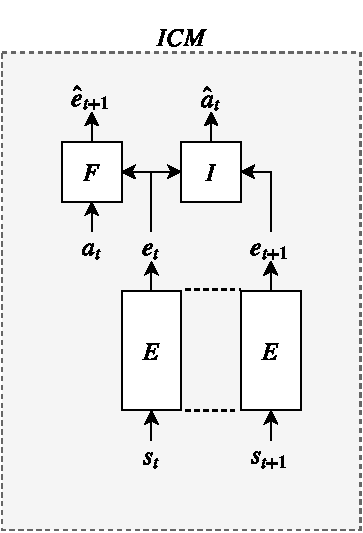
\includegraphics[scale=1]{fig/ICM.pdf}
	\end{center}
		\caption{A schematic representing the intrinsic curiosity module. The module encodes the states $s_t$ and $s_{t+1}$ into encoded vectors $e_t$ and $e_{t+1}$. It uses these vectors in its inverse model $I$ to predict the action taken between $s_t$ and $s_{t+1}$, and it uses the forward dynamics model $F$ to try to predict the encoded next state given the encoded current state and the current action.}
		\label{fig:ICM}
	\end{figure}
	\par The loss for forward model is exactly the intrinsic reward for the agent $r^I$:
	\begin{equation}
		\label{eqn:forward-loss}
		r^I = L(\theta_F) = \mathbb{E} \left[ (\hat{e}_{t+1} - e_{t+1})^2 \right]
	\end{equation}
	and the loss for the inverse model is just
	\begin{equation}
		\label{eqn:inverse-loss}
		L(\theta_I) = \mathbb{E} \left[ (\hat{a}_t - a_t)^2 \right]
	\end{equation}
	\par Recall that, in addition to $I$ minimizing its loss, we also want $E$ to learn an encoding that helps $I$ minimize its loss. Thus, when training $I$ via gradient descent, we let the gradients from $L(\theta_I)$ `flow' back into $E$. We can represent this using the chain rule:\footnote{We average the gradient for the encoder considering it is used twice. The divison by 2 cancels with the multiplication by 2 that results from taking the derivative of the squared-error loss.}
	\begin{align}
		\label{eqn:encoding-loss}
		\nabla_{\theta_E} L(\theta_I) = \mathbb{E} \Big[ (\hat{a}_t - a_t) & \big\vert_{\hat{a}_t = I(e_t, e_{t+1})} \\ & \nabla_{\theta_I} I(e_t, e_{t+1}) \big\vert_{e_{t} = E(s_{t}), e_{t+1} = E(s_{t+1})} \nabla_{\theta_E} \left( E(s_t) + E(s_{t+1}) \right) \Big]
	\end{align}
	and we have a slightly more simple expression for the gradient of just the inverse model:
	\begin{equation}
		\label{eqn:inverse-loss-gradient}
		\nabla_{\theta_I} L(\theta_I) = \mathbb{E} \left[ 2 (\hat{a}_t - a_t) \big\vert_{\hat{a}_t = I(e_t, e_{t+1})} \nabla_{\theta_I} I(e_t, e_{t+1}) \big\vert_{e_{t} = E(s_{t}), e_{t+1} = E(s_{t+1})} \right]
	\end{equation}
	For the gradient of the forward model, we do not let the gradients flow back into the encoding model. This is because the forward model `evaluates' in some sense our encoding function:
	\begin{equation}
		\label{eqn:forward-loss-grad}
		\nabla_{\theta_F} L(\theta_F) = \mathbb{E} \left[ 2 (\hat{e}_{t+1} - e_{t+1})
		 \big\vert_{\hat{e}_{t+1} = F(e_t, a_t)}
		  \nabla_{\theta_F} F(e_t, a_t)
			\big\vert_{e_{t+1} = E(s_{t+1})} \right]
	\end{equation}
	\par The authors of \cite{icm} train a policy $\pi_\theta$ using the reward defined by (\ref{eqn:forward-loss}). The agent is capable of learning to navigate mazes in complex 3D environments to find a goal, where extrinsic reward is conferred only when the agent reaches that goal (and is zero otherwise). Furthermore, adding random noise to the input still results in robust behaviour because the encoding function learns to ignore the noise.

	\subsection{RND}
	\par \cite{rnd} describe a technique called \kword{random network distillation} (RND) that is similar to \cite{icm} in that it uses prediction error as an inrinsic reward signal. However, unlike the ICM, RND does not learn a forward or inverse dynamics model. Instead, the encoding function $E:\mc{S} \to \mc{E}$ is just a randomly initialized neural network called the \kword{feature network} (that is, the encoding is meaningless and serves only as a dimensionality reduction tool). Another neural network called the \kword{predictor network} parametrized by $\theta_f$ learns to predict the output of $E$ The idea is that with training, $f$ will be a good predictor over states that are visited frequently and will be a bad predictor over states that are visited infrequently. The prediction error of $f$ is used as an intrinsic reward signal for the agent.
	\par RND reaches state-of-the-art performance on several Atari games that are considered \kword{hard exploration problems} (where rewards are sparse, require long term decision making, and also require exploration). The authors of \cite{rnd} compared RND to a forward dynamics model by having $f$ try to predict $E(s_{t+1})$ rather than just $E(s_t)$ and found that it performed better than using extrinsic rewards alone, but did not compare specifically to ICM.
	\par As in \cite{icm}, $f$ is trained to minimize the squared error
	\begin{equation}
		\label{eqn:rnd-loss}
		L(\theta_f) = \mathbb{E} \left[\left(f(s_t) - E(s_t) \right)^2 \right]
	\end{equation}
	\par The authors of \cite{rnd} justify their choice by analyzing potential sources of prediction errors:
	\begin{enumerate}
		\item Amount of training data: prediction error is high where few similar examples were seen by the predictor (epistemic uncertainty).
		\item Stochasticity: Prediction error is high because the encoding function is stochastic (aleatoric uncertainty). Stochastic state transitions (such as the noisy tv problem) can cause prediction error in forward dynamics models.
		\item Model misspecification: Prediction error is high because the model class is too limited to fit the target function.
		\item Learning dynamics: Prediction error is high because the optimization process fails to learn to target function.
	\end{enumerate}
	RND uses 1 to encourage exploration. By choosing $E$ to be a deterministic function of the state, we can guarantee that 2 is not part of the prediction error (i.e., we avoid the noisy tv problem). 3 is guaranteed to not be a problem by choosing $f$ to be, for example, a neural network with the same architecture as $E$ but with a different random initialization scheme. In practice, 4 is not a problem since gradient descent is powerful and the encoding function is continuous and stationary.
	\par Importantly, RND was tested with PPO as the policy learning framework, but two value heads were used instead of one in order to allow for different learning rates and scales for $r^E$ and $r^I$.
	\par We use RND as the main intrinsic reward technique to compare against. It is easy to implement, principled, and performs better than forward dynamics models.

	\newpage
	\section{Sparse Distributed Memory}
	\label{sec:sdm}
	\par The main contribution of this thesis is to solve intrinsic reward using a mathematical model of human memory called \kword{sparse distributed memory} (SDM).
	\subsection{RAM}
	\par SDM is generalized version of the \kword{random-access memory} (RAM) that modern computers use to store volatile data while they are running. Numbers on computers are represented as strings of $N$ bits (binary digits, $1$s or $0$s). The number of \kword{addresses} (locations for data) for a given memory is denoted by $M$. A memory with $M=10^6$ could be addressed by $N = 20$-bit words, since $2^{20} = 1,048,576$. At each address, we store some data of size $U$ bits, which we call the \kword{word size}. The capacity of a memory is conventionally defined to be $M \times U$ bits.
	\par RAM comes with three registers: an \kword{address register}, where we input an $N$-bit address $x$, a \kword{word-in register}, where we input a $U$-bit word $w$ we wish to store at address $x$, and a \kword{word-out register}, where we retrieve a $U$-bit word $z$ from address $x$.
	\par Writing to memory consists of providing an address $x$ for the address register and a word $w$ for the word-in register. The data at address $x$ is replaced with $w$. No other addresses in memory are affected.
	\par Reading from memory consists of providing an address $x$ for the address register, from which we read a word $z$ and return this word to the data-out register. We read from a single memory location.
	\par We can represent RAM by
	\begin{enumerate}
		\item $\mbf{A}$: an $M \times N$ matrix of $M$ $N$-bit addresses where each entry along a row is an address in binary,
		\item $\mbf{C}$: an $M \times U$ matrix of $M$ $U$-bit words where each entry along a row is a data stored in RAM, which can be addressed by its row index, and
		\item $\mbf{y}$: a binary vector of length $M$ called the \kword{activation vector} that maps addresses in $A$ to row indices (memory addresses) in $\mbf{C}$. It is 0 everywhere except for the row containing the data in $\mbf{C}$ addressed by a row in $\mbf{A}$.
	\end{enumerate}
	See figure \ref{fig:RAM} for a schematic.
	\begin{figure}[ht]
		\begin{center}
			\textbf{Random Access Memory Schematic}
		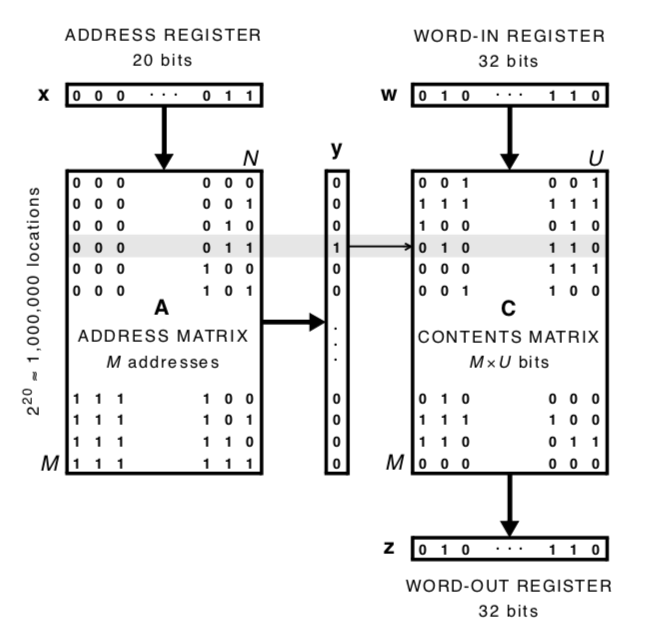
\includegraphics[scale=0.5]{fig/RAM.png}
	\end{center}
		\caption{A schematic representing the layout of RAM. Reproduced from \cite{sdm} with permission.}
		\label{fig:RAM}
	\end{figure}
	\subsection{SDM}
	\par Originally, SDM was developed from the idea that the notion of distance between concepts in our minds (we can say that two concepts are `similar' or `dissimilar') is analogous to the distances between points in high-dimensional spaces.\footnote{The average distance between randomly chosen points in a high-dimensional space under the euclidian metric grows with $O(\sqrt{n})$ where $n$ is the dimensionality of the space.} This should be sufficient to emulate memory and cognition even in the simplest kind of space. For this reason, \cite{sdm} began by using a binary space, where each dimension only contains two elements: $0$ and $1$. Conveniently, this kind of space corresponds to the addresses and also data that are used in RAM. This implies that such a model of memory could be hypothetically be implemented on a machine. However, modern machines have RAM with $N = 32$ or $64$-bit memory addresses. \cite{sdm} states that a high-dimensional space should have hundreds or thousands of dimensions. This is impossible to implement as RAM in reality, since there are around $2^{265}$ atoms in the universe, but we might be interested in having $2^{1000}$ memory addresses or points in our space.
	\par We need to select a \kword{sparse} subset of these points that is representable on a machine. For example, consider trying to model $N = 1000$ dimensions with only $N=20$ bits ($M = 10^6$ \kword{hard locations}, locations in hardware). Then there is a mapping from addresses in the high-dimensional space to hard locations in memory. For simplicity, let us assume that the addresses we wish to use and the data we wish to store are randomly uniformly distributed, and that bits are independent of eachother. Then we may construct such a mapping by randomly sampling $M$ addresses from the high-dimensional space and sending them injectively to a hard memory location.
	\par The problem is that almost certainly no $1000$-bit address sampled randomly from our high-dimensional space is actually represented in our memory mapping. How then should we describe reading from and writing to addresses that aren't implemented?
	\par In typical ram, we activate only a single location in memory for reading or writing ($\mbf{y}$ has a 1 at a single location). In SDM, given an address $\mbf{x}$ to read from or write to, we activate a set of nearby hard locations that are within a certain distance of $\mbf{x}$ ($\mbf{y}$ has a 1 in multiple locations), since $\mbf{x}$ is most likely not represented in $\mbf{A}$.
	\par The notion of distance in a binary space could be euclidian distance, but we typically use the \kword{Hamming distance}, which is the number of places where two words of equal length differ (or for points, the number of dimensions on which their values do not match).\footnote{For example, the Hamming distance between $01101$ and $01011$ is 2} Given an address $\mbf{x}$, we can construct a hypersphere of addresses around it which are less than some Hamming distance $H$ away from $\mbf{x}$ called the \kword{Hamming radius of activation}. Addresses in this hypersphere are considered to be `near' to $\mbf{x}$.
	\par Given an address $\mbf{x}$, we can construct a vector $\mbf{d}$ of distances between $\mbf{x}$ and each address $\mbf{A}_m$ that maps to a hard location. From $\mbf{d}$, we can construct $\mbf{y}$ by setting
	\begin{equation}
		\mbf{y}_m = \begin{cases}
								1 & \mbf{d}_m \leq H \\
								0 & \mbf{d}_m > H
								\end{cases}
	\end{equation}
	See figure \ref{fig:SDM} for a schematic.
	\begin{figure}[ht]
		\begin{center}
			\textbf{Sparse Distributed Memory Schematic} \\
		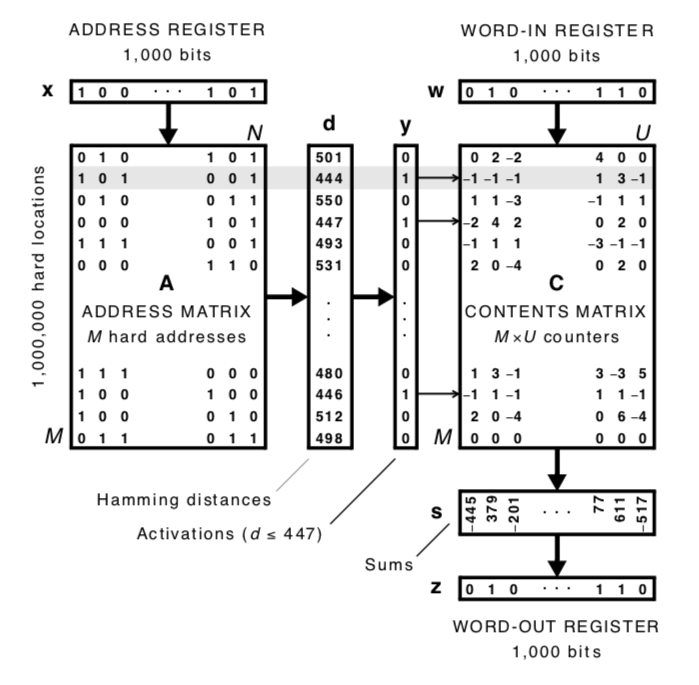
\includegraphics[scale=0.5]{fig/SDM.png}
	\end{center}
		\caption{A schematic representing the layout and function of SDM. Reproduced from \cite{sdm} with permission.}
		\label{fig:SDM}
	\end{figure}
	\par Consider storing a word $\mbf{w}$ at an address $\mbf{x}$ using SDM. Since we will be activating several memory locations, we will write to all of them. However, we do not want to overwrite the data that is stored in these locations. Some of the activated locations might correspond to locations activated by a much different address at some earlier time, and we do not want to destroy that information. Instead, we want to combine the data that we are writing with the data that is stored.
	In typical RAM, $\mbf{C}$ is a matrix of data where each row consists of $U$ bits. In SDM, each row of $\mbf{C}$ is instead made up of $U$ \kword{counters}. When writing a word $\mbf{x}$ to a hard memory location, each counter is adjusted in a bitwise fashion: the counter for each bit is incemented by $1$ if the bit is a $1$, or decremented by $1$ if the bit is a $0$.
	Thus, for some data stored in $\mbf{C}$, if a counter is positive then more $1$s were written to nearby addresses than $0$s. Conversely, if a counter is negative, then more $0$s were written to nearby addresses than $1$s. By writing $\mbf{x}$ to a set of nearby addresses, we \kword{distribute} $\mbf{x}$ to multiple memory locations.
	\par To read a word from an address $\mbf{x}$, we find all nearby addresses $\mbf{A}_m$. Then, for each row in $\mbf{C}$ corresponding to those addresses, we perform an vector summation, producing a vector $\mbf{s}$. Finally, we can produce an output $\mbf{z}$ by thresholding $\mbf{s}$ around $0$:
	\begin{equation}
		\mbf{z}_u = \begin{cases}
								1 & \mbf{s}_u \geq 0 \\
								0 & \mbf{s}_u < 0
								\end{cases}
	\end{equation}
	which essentially performs an inverse of the way we distribute words when writing to memory.
	\par These kinds of computations (checking Hamming distances, making comparisons to thresholds, etc.) can be computationally intensive when done serially, but most of the components of SDM can operate in parallel. This is important, since massive parallelism is one of the important features of the human brain.
	\par It is important to correctly choose the Hamming radius $H$ so that recall maximizes the signal-to-noise ratio of the SDM, where the signal is the word we want to retrieve and the noise is words that have previously been stored nearby. \cite{sdm} demonstrates a comprehensive derivation of the fact that, if storing $T$ words into a memory with $M$ hard addresses, the optimal probability of activating any particular hard address is given by:
	\begin{equation}
		p = \frac{1}{\sqrt[3]{2MT}}
	\end{equation}
	if we model generating hard addresses one bit at a time as a Bernoulli process of $N$ trials with equal probability of choosing a $1$ or a $0$, the resulting distribution is a Bernoulli distribution with mean $\mu = N/2$ and variance $\sigma^2 = N/4$. Since $N$ is large, we can approximate this with a normal distribution with the same mean and variance. If $z(p)$ is the $z$ score for a probability $p$ under a normal distribution, then we can derive an expression for $H$:
	\begin{align}
		\label{eqn:optimal-h}
		H &= \mu + z(p) \sigma \\
		&= \frac{N}{2} + z \left( \frac{1}{\sqrt[3]{2MT}} \right) \sqrt{\frac{N}{4}}
	\end{align}
	For example, given a memory with $M = 10^6$ hard addresses, where addresses have a length $N = 1000$, if we expect to store $T=1000$ words, we get $H = 450$.
	\subsection{Autoassociative Memory}
	\par Why do we care about SDM? What nice properties does it have that can help us solve the problem of intrinsic motivation? It turns out that there are some very interesting uses for SDM when we use data words as address words (that is, $N = U$).
	\par The first case for this is \kword{autoassociative memory}. This means that, when storing a word $\mbf{w}$, we use $\mbf{x} = \mbf{w}$ for the address. Consider storing several noisy copies of some pattern $\mbf{w}$ into the SDM. If we read this word back from memory using $\mbf{x} = \mbf{w}$ for the address, then we get the output word $\mbf{z}$. We can then iteratively read from memory using $\mbf{x} = \mbf{z}$ to obtain a de-noised version of the stored patterns \cite{sdm}. See figure \ref{fig:SDM-denoise-iterative-retrieval} to help visualize this.
	\begin{figure}[ht]
		\begin{center}
		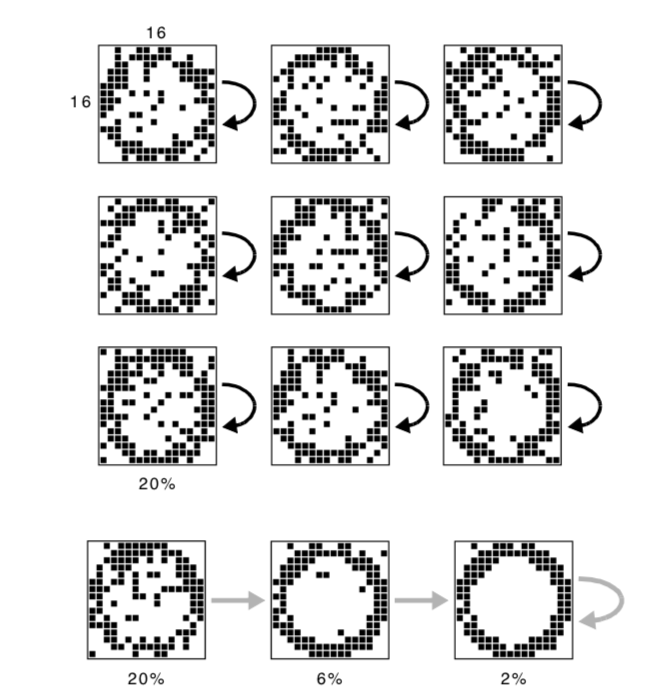
\includegraphics[scale=0.6]{fig/sdm-iterative-retrieval.png}
	\end{center}
		\caption{Using an SDM to store noisy version of a pattern, then iteratively reading from the memory to denoise the stored patterns. We unravel the image into a binary vector of length 256, using this vector as both the address and the data. By repeatedly storing similar data at similar addresses, we store a denoised version that can then be read back from memory. Reproduced from \cite{sdm} with permission.}
		\label{fig:SDM-denoise-iterative-retrieval}
	\end{figure}
	\par The second case for this is \kword{sequential memory}. This means that, given some sequence of words $\mbf{w}_1, \mbf{w}_2, \dots, \mbf{w}_T$, we can store this sequence in the SDM. The idea is to use $\mbf{x} = \mbf{w}_i$ to store the word $\mbf{w} = \mbf{w}_{i+1}$ (that is, use one word as the address for the next word).
	Then to read back this sequence, we do the same process as denoising, where we use the retrieved word $\mbf{z}$ as the address for the next read. See figure \ref{fig:SDM-linked-list} to help visualize this.
	\begin{figure}[ht]
		\begin{center}
		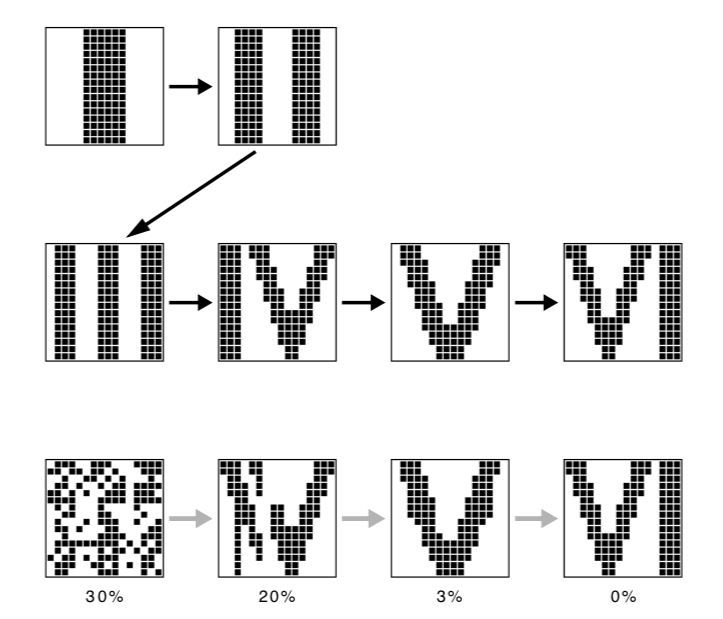
\includegraphics[scale=0.6]{fig/sdm-linked-list.png}
	\end{center}
		\caption{Using an SDM to retrieve a sequence of stored patterns. Given a sequence of data words, we can use the current word as the address for the next word, forming a linked-list. During retrieval, the sequence can be reconstructed by iteratively retrieving a data word and using it as the address to retrieve the next word. Reproduced from \cite{sdm} with permission.}
		\label{fig:SDM-linked-list}
	\end{figure}

	\subsection{Intrinsic Motivation}
	\par The disadvantage of RND is that the reward function is learned. It can take several million timesteps for the predictor network to somewhate accurately predict the output of the feature network, meaning that the intrinsic reward signal is very noisy. This is evidenced by the fact that it took approximately 1.6 billion frames of experience to achieve state-of-the-art performance on Montezuma's Revenge.
	\par Sparse Distributed Memory (SDM) circumvents this. Let us consider some hashing function
	\begin{equation}
		\label{eqn:hash}
		\text{Hash}:\mc{S} \to \{ 0,1 \}^N
	\end{equation}
	that maps states to binary vectors of length $N$.
	\par Consider some binary vector $\mbf{w}$ representing a hashed state. When using autoassociative memory, we use $\mbf{w}$ as the address for writing and reading. Let $\mbf{z}$ be the vector read from memory when using $\mbf{w}$ as an address. If we have written $\mbf{w}$ to memory (or similar data) several times, then the Hamming distance between $\mbf{w}$ and $\mbf{z}$ should be small (close to 0). Otherwise, it should be large (close to $N$). Then we can define the following intrinsic reward signal:
	\begin{equation}
		\label{eqn:intrinsic-reward-sdm}
		r_t^I = \frac{d_H(\mbf{w}, \mbf{z})}{N}
	\end{equation}
	where $d_H$ is the Hamming distance and $N$ is the size of the data words in bits. Then we get a nicely scaled reward that is 0 when we have perfect recall and 1 when we have completely imperfect recall.
	\par By using the autoassociative memory feature of SDM, we can mimic the kind of error used in RND to drive exploration\footnote{We can also use the sequential memory feature of SDM to mimic the kind of forward dynamics error used in ICM. However, this option was not explored due to resource constraints.}. In RND, they use the fact that frequently visited states have lower prediction error as a reward signal. Here, we use the fact that frequently stored words have a lower Hamming distance when read back from memory as a reward signal.
	\par An agent can compute $\text{Hash}(s_t)$ to produce a binary vector $\mbf{w}$. Then, they can read from memory what is stored at address $\mbf{w}$ to get a binary vector $\mbf{z}$. They can then compute the intrinsic reward defined in (\ref{eqn:intrinsic-reward-sdm}).
	\par At some point, the agent will have to write data to memory in order for the reward signal to be meaningful. Deciding when to write to memory is called \kword{write scheduling}.	The choice of write scheduling depends on the choice of hash function and state dynamics.

	\newpage
	\section{Methods}
	\label{sec:methods}
	\subsection{Environments}
	\par One of the most popular environments for testing reinforcement learning agents that work in high dimensional spaces is the \kword{Arcade Learning Environment} (ALE). It is an emulator for the Atari 2600, and includes implementations of several games.
	\par The ALE environments are useful because they provide a consistent interface that can be used by agents, since observations are always the exact same size ($210 \times 160 \times 3$) and all action spaces are discrete. Therefore, it is easy to design a general agent that is capable of, at the minimum, functioning in these environments.
	\par Some ALE environments have sparse rewards. The most popular and one of the most difficult of these is \kword{Montezuma's Revenge}, a 2D exploration and puzzle game. See figure \ref{fig:mr} for an image of the in-game screen. Getting extrinsic rewards requires executing long sequences of moves, exploring unknown areas, and collecting items. It is difficult because rewards are sparse (a random agent takes a significant amount of time to find them), and identifying which actions caused those rewards is generally hard for the agent to learn.
	\begin{figure}
		\begin{center}
			\textbf{Montezuma's Revenge} \\
		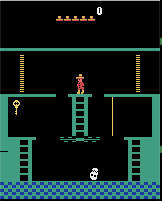
\includegraphics{fig/mr.png}
	\end{center}
		\caption{An image of the starting position of the agent in Montezuma's Revenge.}
		\label{fig:mr}
	\end{figure}
	\subsection{RND as a comparison}
	\par RND achieves state-of-the-art performance in Montezuma's Revenge for a model-free agent with no access to expert demonstrations \cite{rnd}. Because of this, and because of the ease with which RND can be added to an existing reinforcement learning agent, we use RND as a main comparison in this thesis. Here we describe implementation details specific to RND that go beyond the general description of the technique given above.
	\subsubsection{Policy}
	\par The authors of RND use PPO for their policy. PPO has been shown to be largely robust to hyperparameter modifications. PPO is capable of learning both discrete and continuous policies (and for the purposes of their paper and this thesis,  learns a discrete policy). As an actor-critic method, PPO uses two neural networks: one to generate actions (the actor) and one to predict the value of states (the critic).
	\par The authors use a \kword{convolutional neural network} for their policy and for their critic. Convolutional neural networks are neural networks that are specially designed to work well with image-based inputs.
	\par A \kword{convolutional layer} is essentially a function that maps one 3D input (such as the height-width-channels dimensions of an image) to another through the use of \kword{kernels}. A kernel is a \kword{tensor} (which in this case can be thought of as a 3D matrix) of weights, whose last dimension matches that of the 3D input. For example, we might have an image input of size $84 \times 84 \times 4$ and a kernel of size $8 \times 8 \times 4$. We overlay the kernel onto our 3D input and perform a weighted sum of the kernel weights multiplied by the input weights to produce a single value corresponding to the application of that kernel over that area of the input. We then slide the kernel along the input according to its \kword{stride}. In a convolutional layer, we define how many kernels we want to use, and define the kernel size and stride we want to use. The weights of the kernels are part of the learnable parameters of a neural network since the convolution operation is differentiable. We then apply to every value in the output a \kword{nonlinear activation function}.
	\par A \kword{dense layer} or \kword{fully-connected layer} is a layer that maps one vector of inputs to another vector of outputs. We often describe the value of each entry in the vector as being the \kword{activation} of that entry. Thus, a dense layer takes the activations of an input layer and produces activations in an output layer. We can consider each entry in the input layer to be connected to each entry in the output layer with some \kword{weight} that determines how much that input influences that output. We compute the activation for each output by computing a weighted sum of the input activations according to the weights of those connections. Like in convolutional layers, we apply a nonlinear activation function to each value in the output.
	\par We flatten the output of a convolutional layer to feed it into a dense layer since they operate on data of different dimensions. Combining the image-processing power of convolutional layers with the large number of parameters in dense layers makes for a powerful function approximator. We visualize the architecture of the policy network used in figure \ref{fig:policy-architecture}.
	\begin{figure}
		\begin{center}
			\textbf{Policy Architecture} \\
		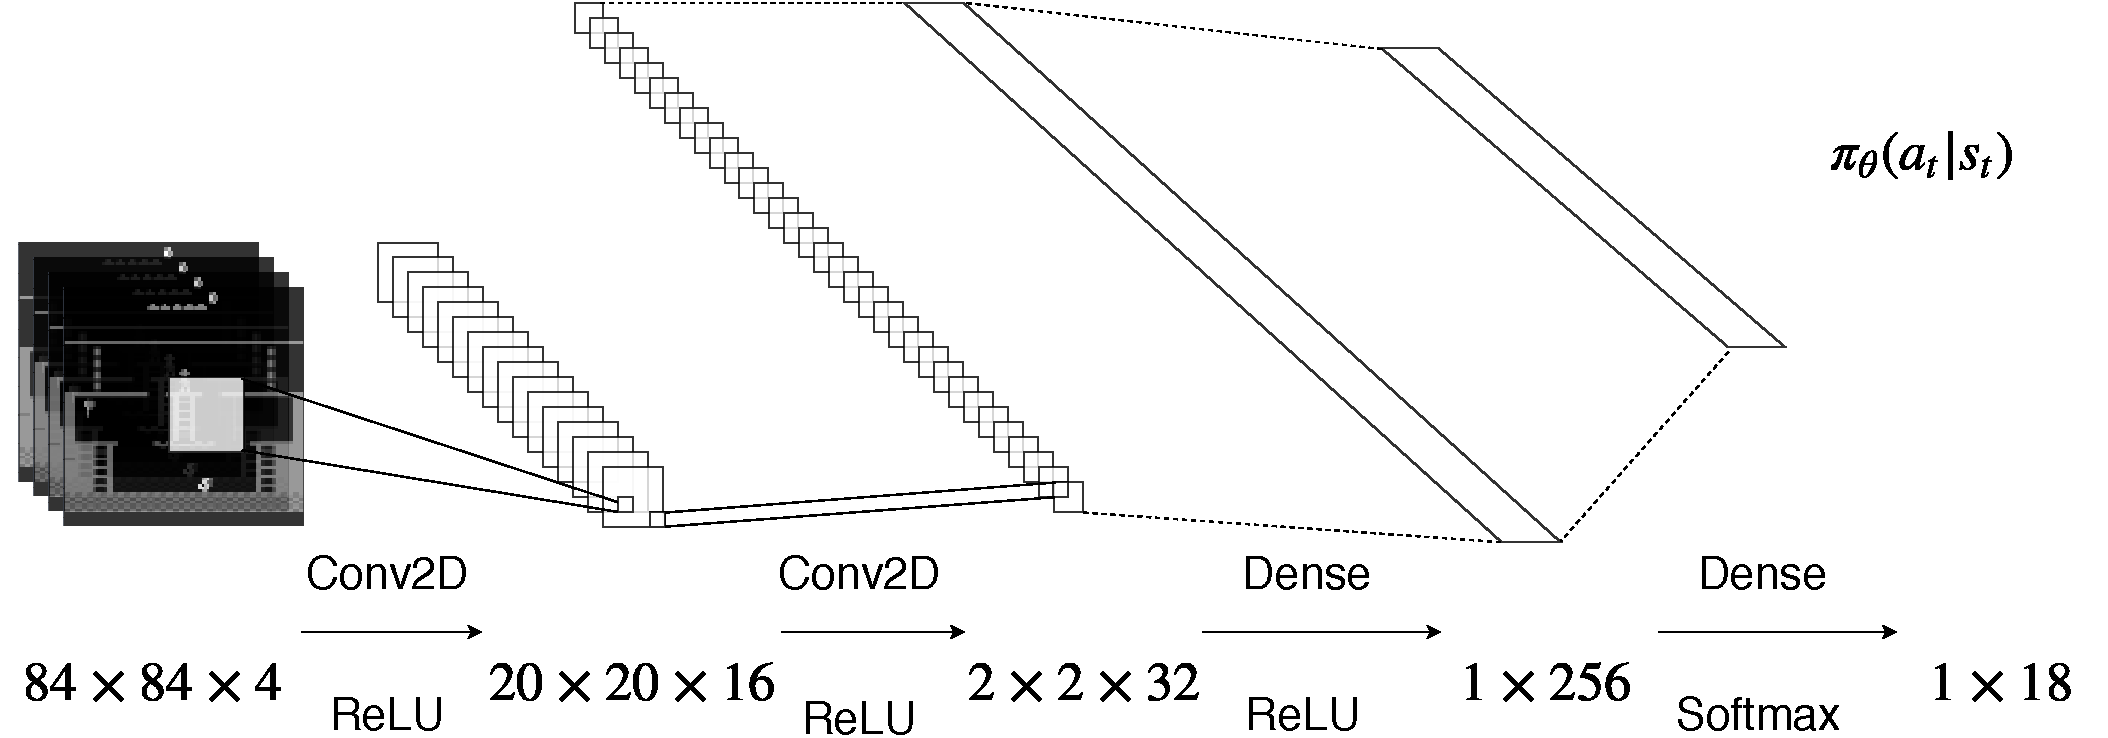
\includegraphics[scale=0.4]{fig/policy-architecture.pdf}
		\end{center}
		\caption{The neural network used as a policy. The inputs are four resized, greyscaled, and framestacked consecutive observations from the environment. The first layer is a convolutional layer that learns 16 kernels of size $8 \times 8 \times 4$ with stride $4$. A ReLU (Rectified Linear Unit) nonlinearity is applied ($\text{ReLU}(x) = \max (0, x))$. The second layer is similar, and learns $32$ kernels of size $4 \times 4 \times 16$ with stride $2$. Again, a ReLU nonlinearity is applied. The output of this layer is flattened into a vector and is connected by a dense layer to an intermediate layer of $256$ outputs, to which a ReLU nonlinearity is applied. Finally, this is connected to an output layer of size $18$ (the number of discrete actions available to the agent) and a softmax nonlinearity is applied to generate a probability distribution from the outputs. A similar network is used for the critic, with the exception that the final layer has a single output rather than $18$, and no activation function is used. This network is exactly the one defined in \cite{rnd}.}
		\label{fig:policy-architecture}
	\end{figure}

	\par The authors use generalized advantage estimation to calculate advantages to optimize their policy.

	\subsubsection{Reward Scale}
	\par While the ALE provides a consistent interface to agents, the scales of rewards can differ from environment to environment. There are different approaches to dealing with this:
	\begin{itemize}
		\item scaling the reward by dividing by a running estimate of the standard deviation
		\item whitening (normalizing) the reward by subtracting a running estimate of the mean and dividing by a running estimate of the standard deviation
		\item clipping the reward within a certain range
	\end{itemize}
	\par The authors of RND chose to clip extrinsic rewards between $-1$ and $+1$. They chose to normalize intrinsic rewards by dividing by a running estimate of the standard deviation. Specifically, normalizing intrinsic rewards handles the fact that the reward distribution is nonstationary. As the predictor network learns to predict the output of the feature network, prediction error decreases. A vanishing prediction error would eventually result in the environment having sparse rewards, defeating the purpose of using an intrinsic reward in the first place.
	\subsubsection{Observation Scale}
	\par The authors do not use raw observations provided by the environment. They modify the observations in different ways depending on whether they are being fed into the policy or whether they are being fed into the predictor network.
	\par All observations are resized to be $84 \times 84$ pixels, and are averaged along the colour channel yielding a greyscale image.
	\par Observations that are fed into the policy (i.e., both the actor and the critic) are scaled to be in the range $[0, 1]$ by dividing by $255$ (since all values in the observations correspond to RGB values). Four consecutive observations are concatenated together in order to provide temporal information to the agent (for example, knowing which way an agent is moving). The final observation is of size $84 \times 84 \times 4$.
	\par Observations that are fed into the predictor network are whitened pixel-wise (after resizing and greyscaling). This is important, since the feature network $E$ and the predictor network $f$ are randomly initialized, and so normalizing observations ensures that the scale of observations has no influence on the ability of the networks to learn, and ensures that the information carried by the features is maximized. Some random initial number of steps are taken to initialize normalization parameters. Unlike the observations fed into the policy, no consecutive frames are stacked. The final observation is of size $84 \times 84 \times 1$.
	\subsubsection{Exploration-Exploitation}
	\par While it is not initially described in \cite{ppo}, in policy gradient methods it is common to use \kword{entropy} as a means of encouraging exploration. Since a policy $\pi$ defines a probability distribution over actions (at least in the discrete case, which we care about here), there is a measure of the uncertainty of the agent:
	\begin{equation}
		\label{eqn:entropy}
		H(\pi_\theta(s)) = -\sum_i \pi_\theta(a_i \vert s) \log \pi_\theta(a_i \vert s)
	\end{equation}
	which achieves a maximum where all actions are equally likely and achieves a minimum when the probability distribution collapses around a single action.
	\par By maximizing entropy, we can ensure that our policy does not converge to choosing a single action too quickly. This prevents us from learning a policy that represents a local maximum, which is difficult to overcome using the methods of gradient descent. It is sufficient to add this to the loss term described in (\ref{eqn:clipped-objective-function}):
	\begin{equation}
		\label{eqn:clipped-objective-function-with-entropy}
		J^\text{CLIP+H}(\theta) = \mathbb{E}_{\pi_\theta} \left[ \min \left( \rho(\theta), \text{clip} (\rho(\theta), 1-\epsilon, 1+\epsilon) \right)  A^{\pi_\theta}(s,a)  + \beta H(\pi_\theta(s)) \right]
	\end{equation}
	where $H(\pi_\theta(s))$ is the entropy of the policy $\pi_\theta$ over discrete actions, and $\beta$ is a parameter that controls the relative importance of the entropy. The authors of RND use $\beta = 0.001$.
	\subsubsection{Combining Episodic and Non-Episodic Rewards}
	\par The authors of RND make an interesting observation: the intrinsic rewards that the agent sees should not be treated episodically (i.e., the time horizon $T$ used for calculating returns should not terminate at the end of an episode). They use the following thought experiment: consider an agent that wants to explore a difficult-to-reach room. If the agent fails, then it dies and the episode ends. Then the cost for that agent of reaching the room should be the cost of playing through an episode to reach that room again, rather than the cost of missed extrinsic rewards. Thus, intrinsic rewards should persist beyond episodes.
	\par This poses a problem, because our critic is only capable of predicting the value of a state $V^{\pi_\theta}(s_t)$ based on the discounted return $G_t$, and the discounted return calculation depends on the time horizon. The solution the authors have is to use a critic with \textit{two} value heads: one for predicting intrinsic (non-episodic) returns and one for predicting extrinsic (episodic) returns. This way, different time horizons can be used for each value head.
	\par The use of two value heads also allows for extrinsic and intrinsic advantage calculations. The advantage of this is that we can compute an overall advantage to optimize the policy using PPO, where the overall advantage is a linear combination of the extrinsic and intrinsic advantages:
	\begin{equation}
		\label{eqn:advantage-linear-combination}
		A = c_I A_I + c_E A_E
	\end{equation}
	where $A_I$ is the intrinsic advantage and $A_E$ is the extrinsic advantage, and $c_I$ and $c_E$ are parameters controlling their relative importance. The authors of RND use $c_E = 2$ and $c_I = 1$.
	\subsubsection{Batched Environments}
	\par When using a complex neural network as the policy (and as a value function estimator), the amount of time spent evaluating the policy can be orders of magnitude higher than the amount of time spent stepping the environment. The difference in cost between outputting a single value in the final layer of a neural network and outputting multiple values in the final layer of a neural network is relatively insignificant. Knowing this, and assuming that environments take less time to simulate than policy evaluation, we can use \kword{batched environments} to accelerate the collection of data for training.
	\par When using batched environments (also sometimes called \kword{vectorized environments}), we replace a single environment with a set of environments. Our policy, given a vector of observations $\vec{s_t}$, generates a vector of actions $\vec{a_t}$ corresponding to the action to be taken in each environment. In return, each environment collectively returns the next observation, together forming a vector $\vec{s}_{t+1}$, and a vector of rewards $\vec{r_t}$. This way, the agent can use the same policy to collect data from multiple environments `in parallel' (though often this means conceptually in parallel, not true parallelism).
	\par The authors of RND note the importance of parallelism and scalability in reinforcement learning, citing its role in the success of modern methods. They also use parallelism as a motivating factor in their design, and criticise the scalability of other intrinsic motivation methods.

	\subsection{Implementation Details for using SDM}
	\par RND was implemented as described by the authors. The advantage of this is that we can do a fair comparison between using RND and SDM by simply replacing the RND calculation of intrinsic reward with that defined in (\ref{eqn:intrinsic-reward-sdm}).
	\par Furthermore, the authors of RND already spent the computational resources on determining which policies and hyperparameters worked best with intrinsic motivation on Montezuma's Revenge. Instead of performing a grid search or randomly sampling hyperparameters from a large search space, we use those found to be optimal by the authors. For a full description of all hyperparameters, see Appendix \ref{app:hyperparameters}.

	\begin{figure}
		\begin{center}
			\textbf{Hash Network}\\
		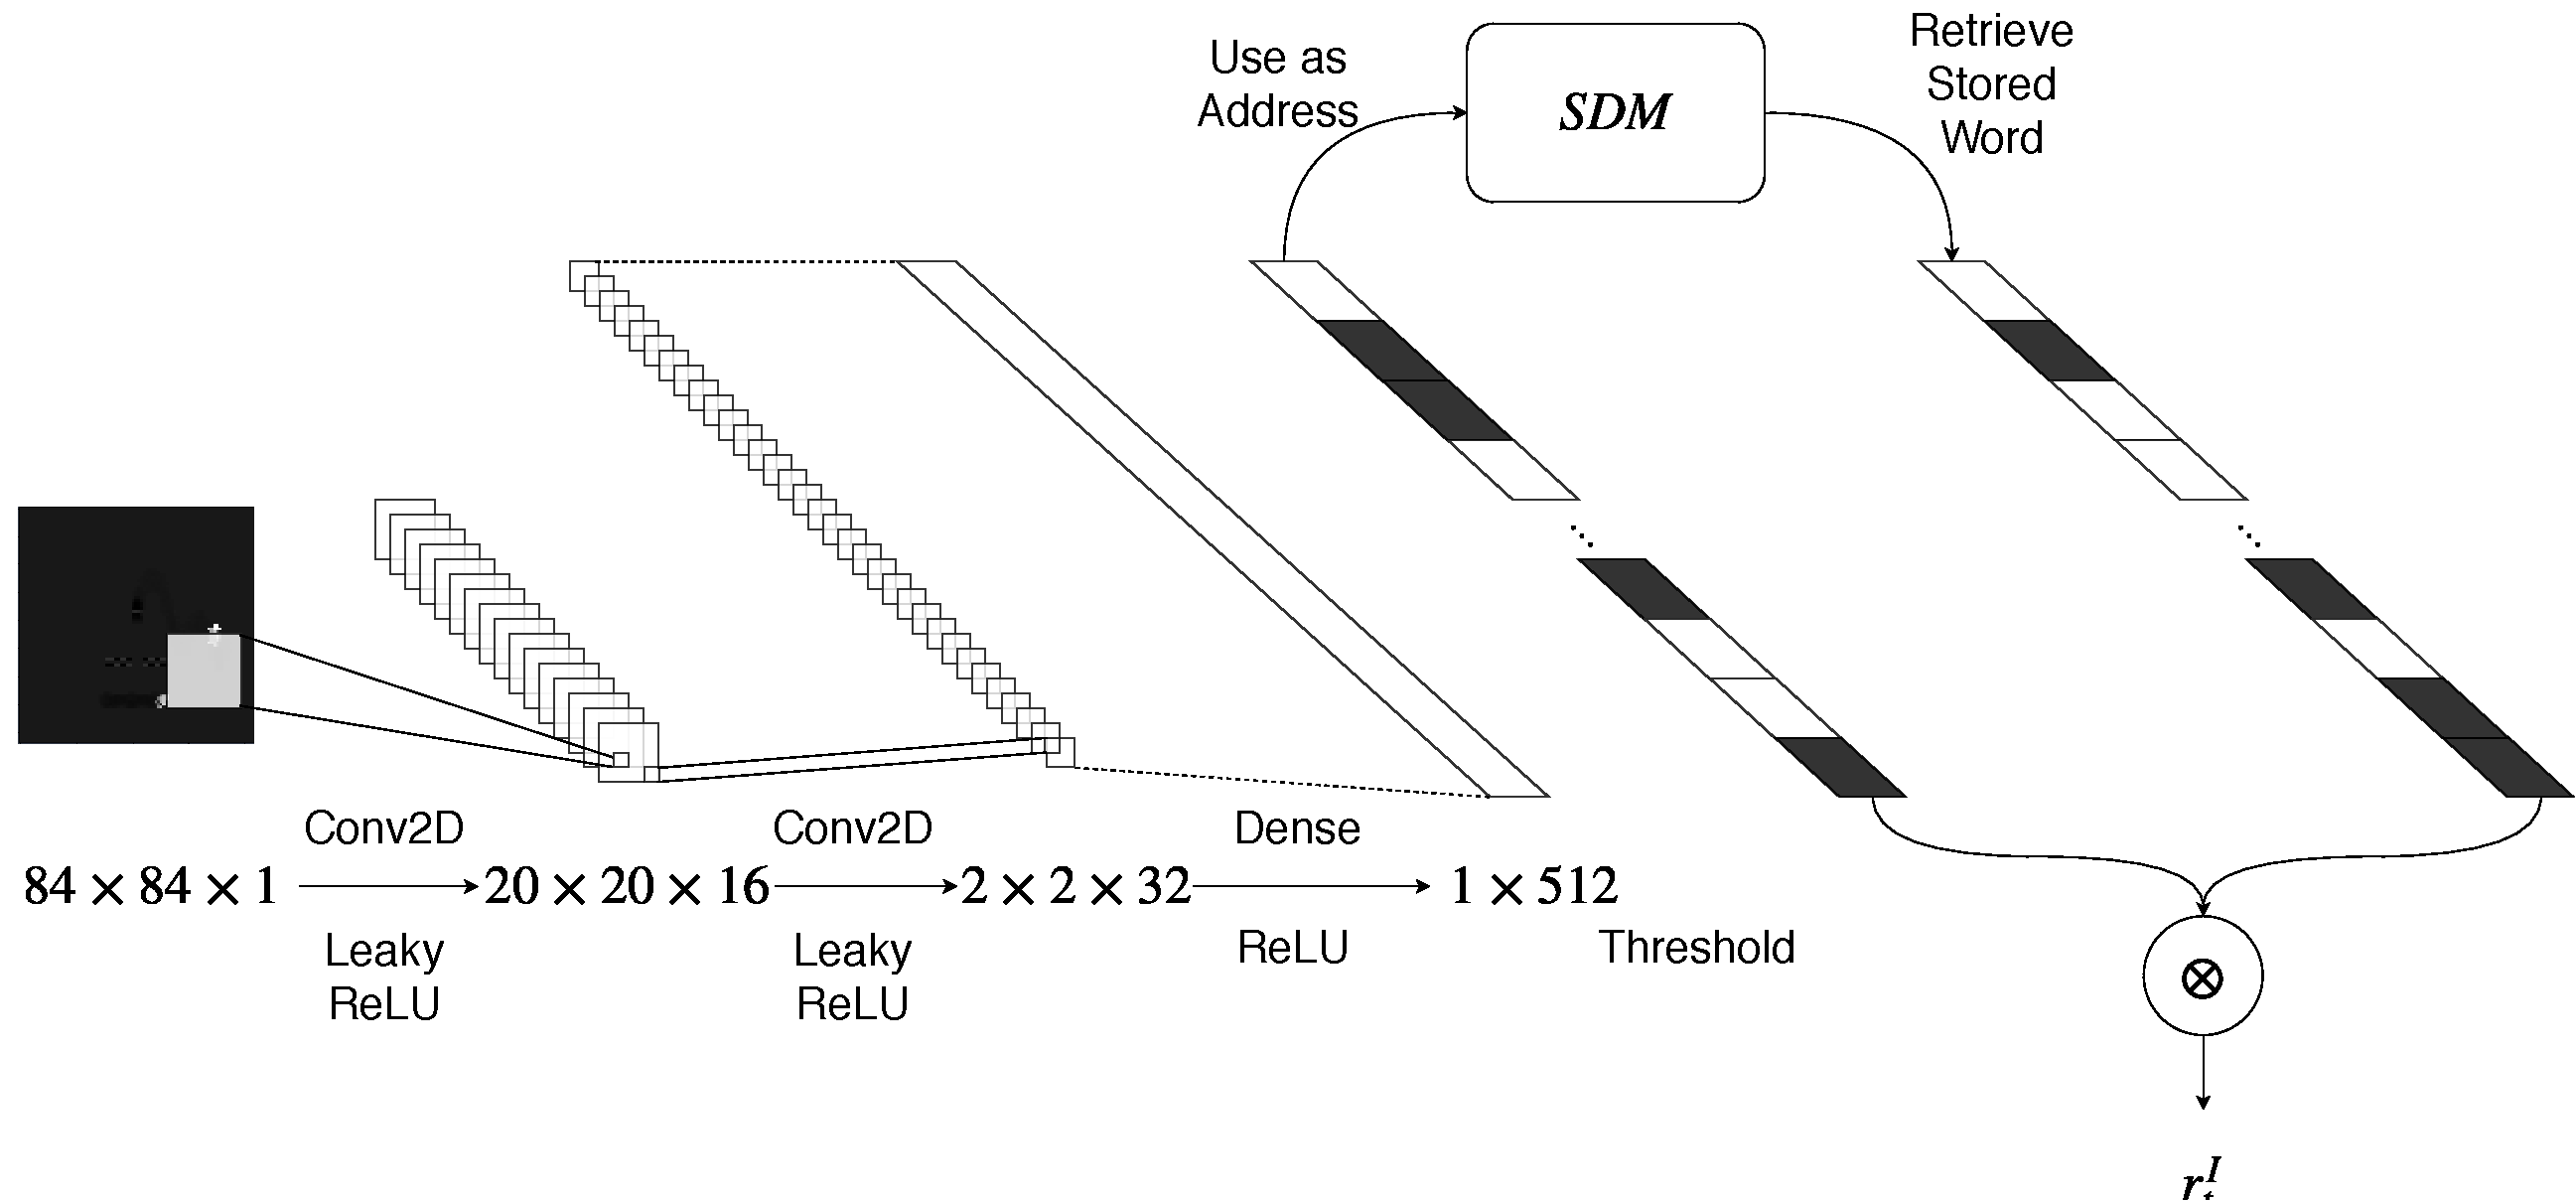
\includegraphics[scale=0.3]{fig/hash-network.pdf}
		\end{center}
		\caption{The hash network used by the agent to map states to binary vectors and to calculate intrinsic reward. It is similar to the policy network from figure \ref{fig:policy-architecture} in architecture, except there is no intermediate dense layer, and the output corresponds to random features. Furthermore, ReLU activations in the convolutional layers are replaced with leaky ReLU activations ($\text{Leaky ReLU}(x) = x \text{ if } x\geq0, 0.01x \text{ if } x<0$). We provide the network with a single resized and normalized observation rather than the framestacked observations used in the policy and the critic. This network is the exact same that is used in \cite{rnd} for generating features, except that no hashing is performed in RND and the output of the last layer is used directly instead.}
		\label{fig:nn-hash}
	\end{figure}
	\par For a hashing function, we use a neural network with the same architecture as the feature network used in RND. A visualization of this is available in figure \ref{fig:nn-hash}. If $o$ is the output of the neural network used for hashing, then we can define the following hash:
	\begin{equation}
		\label{eqn:hash-mean}
		\text{Hash}(s_t)_i = \begin{cases}
												1 & o_i \geq \bar{o} \\
												0 & o_i < \bar{o}
												\end{cases}
	\end{equation}
	which essentially thresholds the output layer around the mean of the output. Figure \ref{fig:hashes-montezuma-revenge} visualizes this hash function for a single environment. Each row of pixels corresponds to the binary vector encoded by the above hash function. Consecutive rows correspond to consecutive timesteps that the agent takes. We can see that the hashes for consecutive timesteps are similar, but not exactly the same, resulting in a noisy vertical banding pattern.
	\begin{figure}[ht]
		\begin{center}
		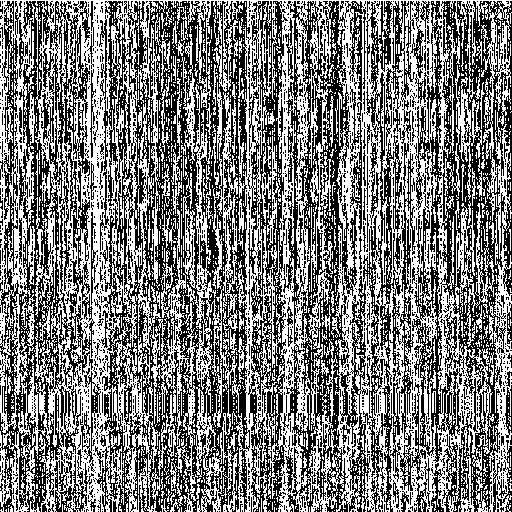
\includegraphics[scale=0.75]{fig/MontezumeRevenge-v0-hashes.jpg}
	\end{center}
		\caption{Hashes for Montezuma's Revenge. Rows correspond to 512 bits computed for the hash. Columns are timesteps. Used $M = 100000, N=512, U=512, T=1000000$ as parameters for the memory.}
		\label{fig:hashes-montezuma-revenge}
	\end{figure}
	\par We use the neural network to produce hashes for multiple batched environments, just as RND uses the neural network to produce feature predictions for multiple batched environments.
	\par The write schedule is quite simple. For a single environment, we could write every timestep, since the hashes are sufficiently different. However, by scaling up the number of environments using batching, we accelerate the rate at which the memory becomes saturated. Thus, we modify the write schedule to write with probability $1/B$ where $B$ is the number of batched environments. This keeps the rate of writing constant, and is equivalent to the strategy that \cite{rnd} uses to decrease the rate of distillation of the predictor network.
	\par Figure \ref{fig:xor-diffs-montezuma-revenge} is a visualization of this write schedule for a single environment. At each timestep, we compute the hash $\mbf{w}$ for the current state, check memory to retrieve a binary vector $\mbf{z}$, and then take their bitwise difference $\mbf{w} \oplus \mbf{z}$.
	\par In figure \ref{fig:xor-diffs-montezuma-revenge}, each row of pixels represents $\mbf{w} \oplus \mbf{z}$. In Montezuma's Revenge, each episode corresponds to using up five lives. The dark bands correspond to timesteps when the agent has fallen to its death, temporarily squirming about on the ground before being reset. During these timesteps, the environment changes very little, and as a result, the agent stores similar information repeatedly in similar addresses. This solidifies the agent's memory of this location, and makes these states less rewarding as a result. It is a happy accident that intrinsic reward decreases upon death, quickly training the agent to avoid dying. Over time, the agent's memory becomes saturated with common hashes, and the differences between computed and retrieved hashes decreases, decreasing the reward of being in those states.
	\begin{figure}[ht]
		\begin{center}
		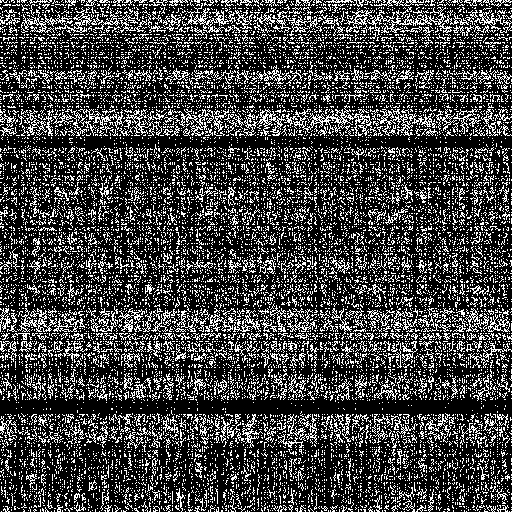
\includegraphics[scale=0.75]{fig/MontezumeRevenge-v0-xor-diffs.jpg}
	\end{center}
		\caption{Bitwise differences between computed hashes and retrieved hashes. Used $M = 100000, N=512, U=512, T=1000000$ as parameters for the memory.}
		\label{fig:xor-diffs-montezuma-revenge}
	\end{figure}
	\subsubsection{SDM Hyperparameters}
	\par There are five hyperparameters available when using SDM:
	\begin{itemize}
		\item $M$: The memory size.
		\item $N$: The size of address words.
		\item $U$: The size of data words. Because we use autoassociative memory, we must have $N = U$.
		\item $T$: The expected number of words to be written.
		\item $H$: The Hamming radius of activation.
	\end{itemize}
	\par Just as RND used 512 features for their embedding, this thesis uses 512 bits for the data word size.
	\par The optimal $H$ computed in (\ref{eqn:optimal-h}) is used under the assumption that my hash function produces sufficiently random bitstrings. Since inputs to the hash network are normalized, and since the weights of the network are randomly initialized, this assumption is fair.
	\par The authors of RND used a total of $30,720,000$ training examples to distill their predictor network into a trained one \footnote{30,000 environment rollouts using 32 parallel environments for 128 timesteps, using $1/4$ of the gathered experience.}. Since our write schedule is analogous to their schedule for training their predictor network, we use $T = 30,720,000$ as our number of expected binary vectors.
	\par We vary the number of addresses $M$, testing performance with $M=10^5, M=10^6$ and $M=10^7$.
	\par The pseudocode for the algorithm is presented in algorithm \ref{alg:pseudocode}, and is adapted from \cite{rnd}.

	\begin{algorithm}
		\label{alg:pseudocode}
		\caption{Training SDM Agent}
	\begin{algorithmic}
		\State $N \gets$ number of rollouts
		\State $N_\text{opt} \gets$ number of optimization epochs
		\State $K \gets$ length of rollout
		\State $t = 0$
		\State sample $s_0$ from $d(s)$
		\For {$i = 1$ to $N$}:
			\For {$j = 1$ to $K$}:
				\State sample $a_t \sim \pi_\theta(s_t)$
				\State sample $s_{t+1}, r_t^E$ from $\mc{P}, \mc{R}$
				\State normalize state $s_t \gets \frac{s_t - \mu}{\sigma}$
				\State compute $\mbf{w} = \text{Hash}(s_t)$
				\State compute intrinsic reward $r_t^I$
				\State normalize intrinsic reward
				\State store $s_t, a_t, r_t^E, r_t^I$ to optimization batch $B_i$
				\State $t = t+1$
			\EndFor
			\State compute $A_E$ and $A_I$ for batch $B_i$ using GAE
			\State compute total advantage $A = c_E A_E + c_I A_I$
			\For {$j = 1$ to $N_\text{opt}$}:
				\State optimize policy using PPO
			\EndFor
		\EndFor
	\end{algorithmic}
\end{algorithm}

	\newpage
	\section{Results}
	\label{sec:results}
	\par The authors of RND already establish that RND exceeds the performance of forward dynamics models like ICM, and consistently surpasses PPO as a baseline with no intrinsic reward. Thus, here we compare only PPO, RND, and SDM.
	\subsection{Reporting Results}

	\subsubsection{Performance}
	\par Several kinds of reporting metrics for policy performance have become popular in reinforcement learning:
	\begin{itemize}
		\item The average score obtained by running the policy in an environment for a fixed number of timesteps, often 18,00 frames which at 60 frames per second for the Atari 2600 environments corresponds to 5 minutes of real-time gameplay \cite{ale}
		\item The improvement in score of the policy over a random agent compared to the improvement in score of a human player ofer a random agent, computed as
		\begin{equation}
			100*\frac{\text{policy score} - \text{random agent score}}{\text{human score} - \text{random agent score}}
		\end{equation} \cite{dqn}
		\item Mean and median performance normalized with respect to some well-performing baseline \cite{ddqn}
	\end{itemize}
	\par We choose to use the following metrics:
	\begin{itemize}
		\item Mean reward obtained by the agent over 18,000 frames, over 5 random seeds. This allows for comparing to published results.
		\item Normalized score with respect to a random baseline. For some environments, a random agent can perform surprisingly well. This allows us to analyze the inductive bias of using reinforcement learning in this environment.
		\item Normalized score with respect to PPO. This allows us to analyze the inductive bias of using an intrinsic reward over relying purely on extrinsic reward.
		\item Normalized score with respect to RND. This allows us to analyze the inductive bias of using a different, faster-convering intrinsic reward signal than the current state-of-the-art.
	\end{itemize}
	\subsubsection{Training Curves}
	\par While final performance of reinforcement learning agents is ultimately how we measure `performance', many existing techniques can peform better if run with a massive number of parallel environments for extremely long periods of time. Thus, we are also interested in the learning dynamics of an agent: how quickly performance increases, and how long it takes behaviour to converge. Part of the motivation for using SDM over RND is that the intrinsic reward signal is useful much more quickly than in RND, which should decrease the number of training samples required to learn good behaviour.
	\par The authors of RND plot the mean cumulative unclipped extrinsic rewards experienced by the agent per episode as a function of the number of parameter updates. This is a simple way to evaluate performance, and allows us to ensure the correctness of our implementation.
	\par These training curves are often plotted as the average over all parallel workers, with shaded regions representing the standard deviation in performance. Because training in reinforcement learning is not always highly stable, the performance is often smoothed by taking the mean across a window of a fixed number of timesteps. The authors of RND do not disclose the size of their smoothing window used in plotting, but we use 10 here.
	\subsection{Varying SDM Parameters}
	\par Due to the success of RND, we took the best-performing hyperparameters from RND and used them when applying SDM. This was partially done due to computational constraints; large-scale reinforcement learning research often uses clusters of GPU-accelerated machines, which were not available for this thesis. Resource limitations prohibited the use of a grid search on the wide variety of hyperparameters available, but also ensured a fair comparison between algorithms. Furthermore, as a general principle of reinforcement learning research, a method should be highly robust to hyperparameter changes.
	\par Consequently, the only hyperparameter that was modified was the size of the memory $M$. Table \ref{tbl:results} shows the results of a trained agent after $480,000$ parameter updates\footnote{$30,000$ rollouts, each with 4 minibatches, updated for 4 optimization epochs}.
	\begin{table}[ht]
		\begin{center}
	\textbf{Performance of Trained Algorithms} \\ \medskip
	\label{tbl:results}
	\begin{tabular}{c |p{2cm} p{2cm} p{2cm} p{2cm}}
		$M$ & Cumulative Reward & RND-Normalized & PPO-Normalized & Random-Normalized \\ \hline
		$10^5$ & $3607 \pm 651$ & $45.82\%$ & $141.45\%$ & $13035\%$\\
		$10^6$ & $3553 \pm 428$ & $45.15\%$ & $139.33\%$ & $17765\%$\\
		$10^7$ & $4251 \pm 399$ & $54.01\%$ & $166.71\%$ & $21255\%$\\
		\hline
		RND & $7871 \pm 676$ & & & \\
		PPO & $2550 \pm 0$ & & & \\
		Random & $20 \pm 40$ & & & \\
	\end{tabular}
	\end{center}
	Mean cumulative extrinsic reward in Montezuma's Revenge over $18,000$ frames of experience at $60$ fps (about 5 minutes of real-time gamplay). Performance measured after $480,000$ parameter updates, except for random agent. 5 rollouts were used for testing, each with a random period of 0 to 100 frames where the agent did not perform any actions.
	\end{table}
	\par The most important result from this experiment is that SDM is capable of improving performance over a competitive baseline reinforcement learning algorithm by supplementing extrinsic rewards with intrinsic rewards. Applying SDM with any memory size performs significantly better than PPO\footnote{The PPO agent found the exact same sequence of rewards over all $18,000$ timesteps on all 5 runs, resulting in a standard deviation of zero. Significance testing is not exactly meaningful here.}.
	\par Unfortunately, using SDM does not achieve state-of-the-art performance. Our agent is capable of playing Montezuma's Revenge at approximately an amateur human's level of play \cite{rnd}.
	\par Compared to a random agent, which only found a single extrinsic reward of 100 across 5 random seeds, all agents perform extremely well. This comparison is not meant to show relative improvement, but rather to demonstrate the extreme sparseness of extrinsic rewards. In some environments, random agents can perform almost as well as (or even better than) reinforcement learning algorithms \cite{rnd}.
	\par Increasing memory size from $10^5$ to $10^6$ did not change performance significantly. Further increasing memory size to $10^7$ improved performance somewhat, though this difference is not statistically significant ($t=1.88, p=0.09$).
	\par We visualize the training process in figure \ref{fig:training-curve}. The training curves for PPO and for RND look similar, but not exactly the same as \cite{rnd}, confirming the correctness of its implementation. The random agent generally fails to find any positive reward, and when it does, averaging across environments causes these rewards to be diminished.
	\par All agents initially begin to learn quickly and at similar rates, with $M=10^7$ SDM being competitive with RND up until approximately $250,000$ parameter updates. By viewing the RND agent, we found that this increase in extrinsic reward occurred when the agent learned to access a room that had further easy access to adjacent rooms. The SDM agents did not find this room. Because of computational resources, these training curves represent a single run of training agents. As a result, it cannot be certain if RND's choice to move to this new room happened randomly, or would have happened consistently across runs.
	\par While PPO initially learns quickly, once it learns to acquire all of the extrinsic rewards that it can easily find, it exploits finding these rewards and has great difficulty stumbling into further rewards. Both RND and SDM surpass PPO in performance relatively early on.

	\begin{figure}[ht]
		\begin{center}
		\textbf{Comparison of Algorithm Performance with respect to Training} \\
		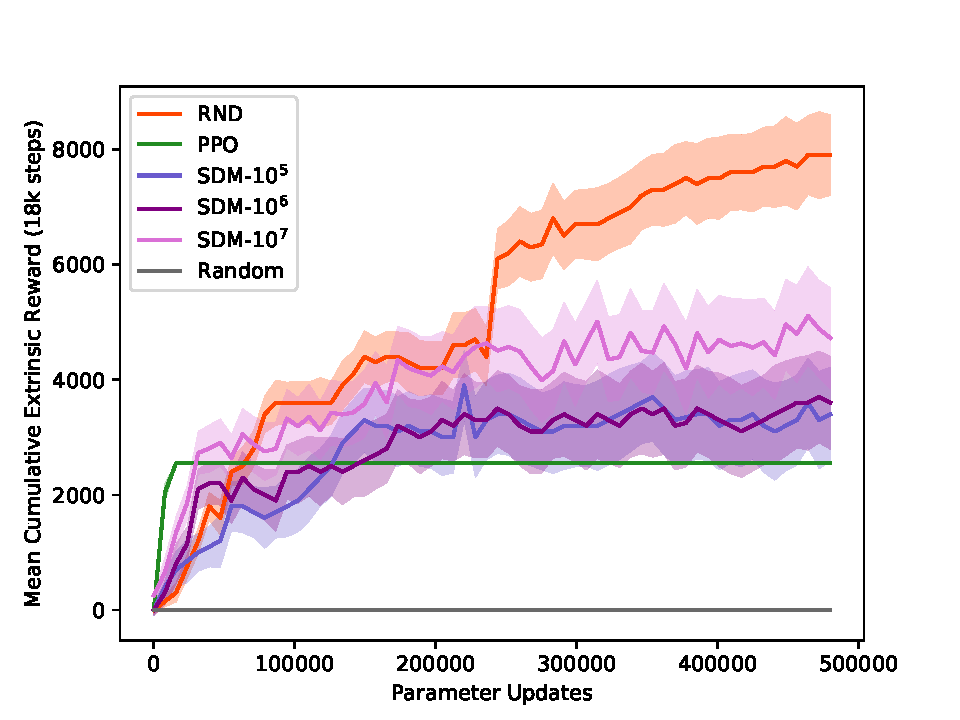
\includegraphics{fig/training-curve.pdf}
	\end{center}
		Mean cumulative extrinsic reward over training episodes (18,000 steps or when the agent uses up five lives, whichever happens first). Averaged over 32 parallel environments. Shaded region represents standard deviation. $X$ axis is parameter updates. RND: Random Network Distillation. PPO: Proximal Policy Optimization. SDM-$M$: Sparse Distributed Memory with specific memory size $M$. Random: Agent whose policy is to sample actions uniformly randomly from the action space.
		\label{fig:training-curve}
	\end{figure}

	\newpage
	\section{Discussion}
	\label{sec:discussion}
	\subsection{Limitations}
	\par Before undertaking this thesis, the author had some understanding of how reinforcement learning worked, and had some experience using neural networks in the context of supervised learning. However, the author did not fully understand the resource requirements for research-level reinforcement learning.
	\par The first resource that was limited was computational resources. Groups that are ubiquitous in the reinforcement learning literature have access to large clusters of GPU-accelerated machines, which allow for rapid protototyping of agents. Furthermore, they allows for parallel data collection and parallel hyperparameter testing. The data collected in this thesis used a single laptop with a two-core CPU and no GPU, which slowed development considerably.
	\par Furthermore, for problems with complex state-spaces, like Montezuma's Revenge, it can take millions or billions of timesteps of experience for an agent to show learning. As a result, debugging programs often required a significant amount of patience to tell if the agent was learning or not. This, coupled with time limitations, limited the amount of experiments and testing that was feasible. It also limited the ability to run long-running experiments over several random seeds, since each would take up to several days to complete.
	\par The limitations on resources leads to a degree of uncertainty in the results, since only a single random seed for policy initialization was used for each algorithm. Furthermore, the agents that were trained over a single run were then used to evaluate the learned policy. Thus, it is possible that over a larger number of random seeds, results could have varied. Because the final performance of the RND agent matched published results, the author is at least partially confident that the RND is performing as well as expected. However, it is possible that with additionaly hyperparameter tuning and network architecture choices, among other things, that SDM could outpeform RND.
	\subsection{Reasons for Performance}
	\par SDM performs better than PPO but worse than RND. Originally, we theorized that RND's slow convergence as a reward signal meant that it took a significant amount of time to generate good performance. We believed that the more instantaneous nature of the reward signal from SDM would be beneficial to the agent, very quickly telling it whether it was in a novel state or not.
	\par Recall the agent uses the \kword{advantage} of choosing certain actions in certain states to decide whether or not those actions are good. For both RND and SDM, the agent's actions should incur a negative intrinsic advantage when visiting common states, such as the starting position of the agent, to which the agent is set at the beginning of every episode and after losing a life. The reward for being in this state consistently decreases over time, as it becomes more and more familiar to the agent. However, the rate at which states become familiar to the agent is important for exploration. For RND, the slow rate of convergence of the reward signal is actually beneficial; each time the agent begins an episode, the difference in prediction error is only slightly smaller than before, making that state only slightly less novel to the agent, thus not incurring a large negative advantage. When using SDM however, the agent learns in only a few episodes that the starting state is not novel, and quickly begins to confer 0 intrinsic reward as perfect recall of hashes is achieved. As a result, SDM intrinsic rewards become sparse relatively quickly compared to RND, whose reward signal changes more slowly. As the returned rewards decrease, the agent experiences a negative advantage, discouraging whatever actions were taken at the start of an episode. This process repeated over time leads to an agent that chooses random actions in common states, since all actions are equally bad. Once intrinsic rewards stabilize to zero this effect goes away. Because intrinsic rewards dissipate like this, any actions taken in common states have no influence on the overall return or advantage for a rollout, and the agent only learns which actions are good based on their eventual outcome. However, since rollouts are only of length 128 for a single environment, this requires that an agent find some intrinsic reward within 128 timesteps, which can sometimes be difficult since many of the states encountered at the start of an episode or after respawning from a death are going to be very common to the agent. The resulting reward signal after acquiring experience is one that is slightly sparse; not as sparse or as difficult to achieve as the true extrinsic reward, but not as a dense as that of RND.
	\par When examining the average intrinsic reward recieved by SDM agents over time, the intrinsic reward signal evaporates entirely to zero at around $300,000$ timesteps. After this point, the agent is essentially learning using only PPO, since it is operating entirely based on extrinsic rewards. However, having gained enough experience to learn how to get easier rewards from earlier in the game using SDM, the agent still manages to outperform PPO.
	\par There seems to be an improvement in performance when increasing the memory size. It is not exactly clear what the relationship is between memory size and performance. Recall that addresses are sampled randomly from our address space of $\{0, 1\}^N$ under the assumption that the data to be stored is random. We compute our Hamming radius of activation based on the number of addresses and the optimal probability of activating a random address, but changing $M$ does not significantly alter the radius of activation. For $M=10^5$ we get $H=212$, for $M=10^6$ we get $H=210$ and for $M=10^5$ we get $H=208$. For each memory size, the intrinsic reward tends to dissipate at around the same time. As such, it is likely that the difference in performance is simply due to random seed, with the agent stumbling into extrinsic rewards randomly.
	\subsection{Future Work}
	\par Beyond using additional resources to test out basic hyperparameters and network architectures, there are some directions for future work that may be beneficial.
	\par While RND has been shown to outperform dynamics-based methods \cite{rnd}, this class of methods still has merit for intrinsic reward. For example, the authors of RND did not test RND in a visually complex 3D environment, and did not implement their forward dynamics model exactly as described in referenced papers. Thus, there is the possibility that SDM can work well in other environments. It is possible to easily extend SDM to use forward dynamics error using the sequential memory property of SDM. By comparing the recalled hash for the next state with the evaluated hash for the next state, using the hash for the current state as the address, we can generate a kind of prediction error common to all dynamics-based models of intrinsic reward.
	\par Additionally, it would be interesting to measure the influence of using a write schedule that only writes hashes to memory if a state is considered sufficiently novel. This would attenuate the rate of memorization that the agent undergoes, rather than continually writing states to memory at every time step.
	\par While we focused on using PPO and policy gradient methods here, it would be interesting to know if one can extend the notion of two value heads for the critic in PPO to two value heads for the $Q$-network in deep $Q$-learning. Currently, even the most advanced DQNs fail to obtain significant rewards in Montezuma's Revenge \cite{rainbow}.
	\par PPO can be used with continuous action spaces using diagonal Gaussian distributions. DDPG is built specifically for continuous action spaces. It could be beneficial to see if either RND or SDM can achieve good performance in sparse reward environments with continuous action spaces.
	\par Montezuma's Revenge, despite having a \textit{large} observation space, does not have a highly \textit{complex} observation space. It is possible that a complex 3D environment would be too difficult for RND to learn, with inputs varying too much for the predictor network to learn. In this case, the rapid convergence of SDM may  benefit the agent more than RND.

	\newpage
	\section{Conclusion}
	\label{sec:conclusion}
	\par Reinforcement learning is a fascinating field that has come very far in recent years. Reinforcement learning does especially well in environments with dense rewards, but struggles when rewards are sparse. This thesis considers some possible solutions to the sparse reward problem, focusing on random network distillation, and a novel proposed algorithm that leverages sparse distributed memory to measure novelty. We find that using sparse distributed memory can improve the performance of an agent that relies only on sparse extrinsic rewards. While this approach does not exceed state-of-the-art performance, it validates the use of SDM as a tool for measuring novelty and guiding exploration. Using SDM is a promising approach with a rich set of directions for future study.
	\newpage
	\bibliographystyle{apalike2}
	\bibliography{references}

	\newpage
	\begin{appendices}
		\section{Hyperparameters}
		\label{app:hyperparameters}
		\begin{table}[ht]
		\centering
		\label{tbl:hyperparameters}
		\begin{tabular}{c |c}
			\hline
			Training & \\
			\hline
			Rollouts ($N$) & $30,000$ \\
			Optimization Epochs ($N_\text{opt}$) &  $4$\\
			Rollout Length ($K$) & $128$ \\
			Number of minibatches & $4$ \\
			\hline \hline
			PPO & \\
			\hline
			Learning Rate & $0.0003$ \\
			Entropy Coefficient ($\beta$) & $0.001$ \\
			Optimizer & Adam \\
			Extrinsic Advantage Coefficient ($c_E$) & 2 \\
			Intrinsic Advantage Coefficient ($c_I$) & 1 \\
			$\gamma_I$ & $0.99$ \\
			$\gamma_E$ & $0.999$ \\
			$\lambda$ & $0.95$ \\
			Clip range ($\epsilon$) & 0.1\\
			\hline \hline
			RND & \\
			\hline
			Number of features & $512$ \\
			Proportion of experience used for training & $1/4$ \\
			\hline \hline
			SDM & \\
			\hline
			Memory Size ($M$) & $\{10^5, 10^6, 10^7 \}$ \\
			Expected number of data ($T$) & $30,720,000$ \\
			Word Length ($N = U$) & 512\\
		\end{tabular}
		\end{table}

	\end{appendices}
	\null
  \thispagestyle{empty}%
  \newpage
	\null

\end{document}
